\chapter{Vergleich mit anderen Computer Vision Applikationen}
\label{sec:rectification}


Ein weit verbreiteter Ansatz der Stereobildanalyse basiert auf zuvor Rektifizierten Bildern. Rektifizierte bilder zeichnen sich dadurch aus, dass die jeweiligen Epipole der Bilder ins unendliche projiziert werden, was dazu fürhrt, dass die jeweiligen Epipolarlinien der Bilder parallel zueinander verlaufen. Anschließend werden die Epipole noch so rotiert, dass die Epipolarlinien in einheitlichen Scanlinien über beide Bilder verlaufen. In Abbuldung \ref{fig:Scanlinien} ist das graphisch dargestellt\cite{Fusiello,Javier,ZZ,MatlabRec,phdextrinsicPara}.

\begin{figure}[!htb]
	\centering
	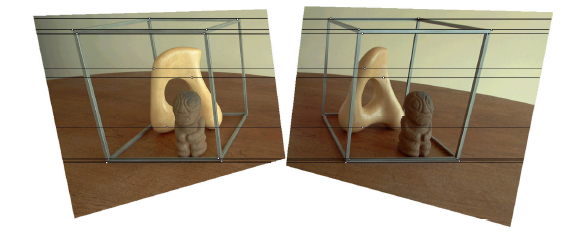
\includegraphics[width=.8\linewidth]{images/rectifiziertesBildAusZZ.png}
	\caption[Beispiel eines Rektifizierten Bildes mit Scanlinien]{Beipiel eines rektifizierten Bildes. Die Epipole beider Bilder sind ins unendliche projiziert worden. Des Weiteren wurden die Epipol so rotiert, dass die Epipolarlinen zu einheitlichen Scanlinien über beide Bilder verlaufen. Quelle: \cite{ZZ}} 
	\label{fig:Scanlinien}
\end{figure}

% parallelen Epipolarlinien anschließend noch zu einheitlichen Scanlinien über beide Bilder entlang einer Koordinatendachse ausgerichtet werden.
 
Anhand der so entstandenen Scanlinien, wird die Suche nach weiteren korrespondierenden Punkten auf eine eindimensionale Suche beschränkt, da nur noch entlang der entsprechenden korrespondierenden Epipolarlinie gesucht wird. Die Rektifizierung, macht es somit möglich die Bildpunkte kompletter Bilder mit relativ geringem Rechenaufwand zu rekonstruieren\cite{ZZ,Fusiello,Javier}. Jedoch verlangen viele Rektifizierungsansätze als Voraussetzung, dass das verwendetet Stereobildpaar die selbe Auflösung besitzt.\\

Der in dieser Arbeit entwickelte Szenenrekonstruktionsalgorithmus wurde so entwickelt, dass eine Rektifizierung der Bilder, nicht notwendig wird. Der Grund dafür ist, dass ein Algorithmus entsteht, welcher auch mit Bildern unterschiedlicher Kameraauflösungen eine erfolgreiche Rekonstruktion vollbringt.\\

Im verlauf des Kapitels wird zunächst der Arbeitsprozess der Stereoanalyse auf Basis von Bildrektifizierungen erläutert. Anschließend wird ein Rektifizierungsalgorithmus nach \cite{ZZ} vorgestellt werden, welcher nur durch Vorwissen von 9 korrespondierenden Punkten und der daraus resuliterenden Fundamentalmatrix eine Rektifizierung zweier Bilder ermöglicht. Der Rektifizierungsalgorithmus wurde anhand des synthetischen Stereoaufbaus aus Kapitel \ref{sec:minimal} implementiert. Mit dem so entstandenen Algorithmus werden zunächst zwei Bilder gleicher Auflösung rektifiziert und danach werden zwei Tests mit Bildern unterschiedlicher Auflösung aufgezeigt und analysiert.


%Eigener Ansatz implementierung eines Rektifizierungsalgorithmus zum test auf Funktionaliät unter schiedlicher Aflösungen \\
%
%Ergebnisse Präsentieren\\

\section{Szenenrekonstruktion mit Rektifizierung}


Da bestimmte Formen der Rektifizierung keine vorherige Kalibrierung der Kameras benötigen, wird diese Methode in den meisten gängigen Echtzeit-Szenenrekonstruktionen eingesetzt. \cite{Fusiello,Javier,R.H.}. Der Arbeitsprozess für die Szenenrekonstruktion auf Basis von rektifizierten Bildern, welcher in Abbildung \ref{fig:ArbeitsprozessRektifizierung} schematisch dargestellt ist, unterscheidet sich etwas zu den bereits bekannten Arbeitsprozessen, welche in den Abbildungen \ref{fig:ArbeitsProzessVirtuell} und \ref{fig:ArbeitsProzessReell} zusammengefasst sind.\\


\begin{figure}[!htb]
	\centering
	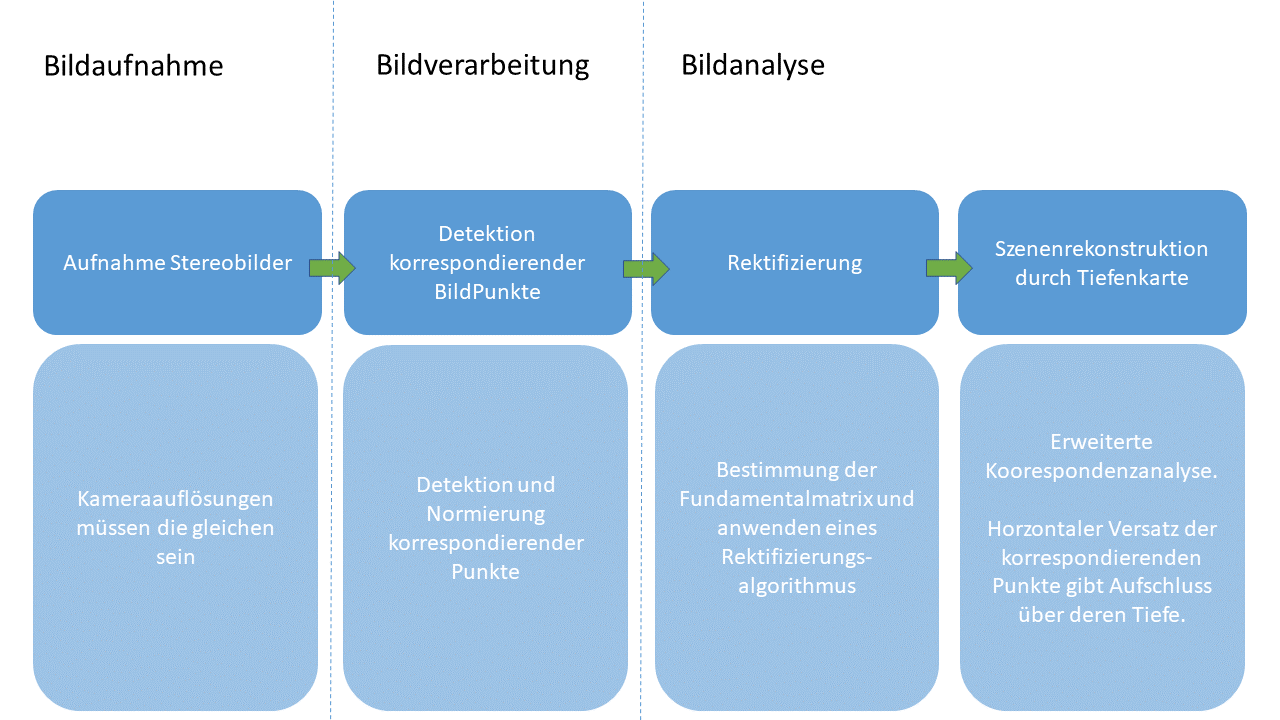
\includegraphics[width=.8\linewidth]{images/NEU_Rektifizierung_Arbeitsprozess.png}
	\caption[Arbeitsprozess der Szenenrekonstruktion mit Rektifizierung]{Ablaufdiagramm der Szenenrekonstruktion basierend auf einem Rektifizierungsansatz} 
	\label{fig:ArbeitsprozessRektifizierung}
\end{figure}


Der entscheidende unterschied zwischen den beiden Ansätzen liegt im Abschnitt der Bildanalyse. Es wird davon ausgegangen, dass die intrinsischen Kameraparameter im einzelnen nicht bekannt sind. Der Ansatz beinhaltet auch keinen Kalibrierungsschritt, in welchem intrinsische oder extrinsische Kameraparameter bestimmt werden sollen. Das Ziel, des in Abbildug \ref{fig:ArbeitsprozessRektifizierung} gezeigten Ansatzes, ist es eine 3D-Szene mit möglichst wenig Informationen aus einem Stereobildpaar zu rekonstruieren \cite{ZZ,Javier,Fusiello,phdextrinsicPara}.\\

Zunächst werden acht bis neun korrespondierende Punkte in einem Stereobildpaar detektiert. Aus den zuvor noch, wie in Kapitel \ref{sec:real} beschriebenen, normierten korrespondierenden Punkten wird eine Fundamentalmatrix $F$ bestimmt. Aus den korrespondierenden Punkten und der Fundamentalmatrix $F$ wird ein Rektifizierungsalgorithmus, wie beispielsweise in Kapitel \ref{sec:Rektifizierungsalg}, angewandt, welcher zwei Stereobilder so transformiert, dass ihre Epipolarlinien zu horizontal ausgerichteten Scanlinien werden, wie in Abbildung \ref{fig:Scanlinien} zu sehen ist.\\

Mit Hilfe dieser entstandenen Scanlinien, wird die Suche nach weiteren korrespondierenden Punkten von einer zweidimensionalen auf eine eindimensionale Suche runter gebrochen, da sich diese jeweils entlang der zum Punkte entsprechenden korrespondierenden Epipolarlinien befinden\cite{ZZ,Fusiello,Javier}. \\

Es wird davon ausgegangen, dass die Bilder aus zwei verschiedenen Blickwinkeln aufgenommen wurden. Nach der Rektifizierung ist zwischen zwei korrespondierenden Punkten ein horizontaler Versatz zu verzeichnen, wie in Abbildung \ref{fig:DisparityMap} in den ersten beiden Bilder zu sehen ist. Dieser Versatz entsteht durch den Abstand der beiden Kameras zueinander. Der Versatz zwischen den beiden korrespondierenden Punkte wird als Disparität bezeichnet. Je weiter ein Objekt von den Kameras weg ist, desto geringer ist die zu verzeichnende Disparität\cite{Javier}.\\

Bei der Disparität handelt es sich um einen numerischen Wert. Diesem Wert kann je nach Größe ein Grauwert zugeordnet werden. Je größer eine Disparität zwischen zwei Punkten ist, desto heller wird der entsprechende Grauwert gewählt und je geringer die Disparität desto dunkler wird der Grauwert. Anhand der zugeordneten Grauwerte kann ein Bild generiert werden, welches auch als Disparitätskarte oder Tiefenkarte bezeichnet wird\cite{Javier,MatlabDisp}. Diese Disparitätskarte gibt ein Maß für die Tiefe der Objekte in der Szene an\cite{Javier,MatlabDisp}.

\begin{figure}[!htb]
	\centering
	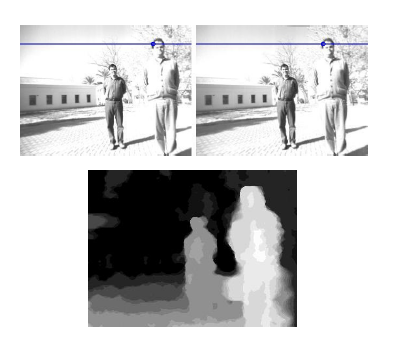
\includegraphics[width=.8\linewidth]{images/Disparity.png}
	\caption[Entstehung einer Disparitätskarte]{In den oberen beiden Bildern sind in blau zwei korrespondierende Epipolarlinien zu sehen, die zusammen eine Scanlinie bilden. Im Bild darunter ist eine aus den Dispritäten zweier Bilder zueinander entstandene Disparitäts beziehungsweise Tiefenkarte zu sehen. Quelle: \cite{Javier}} 
	\label{fig:DisparityMap}
\end{figure}

Voraussetzung für dieses Verfahren ist es jedoch, dass beide Bilder mit Kameras gleicher Auflösung aufgenommen wurden. Bei unterschiedlichen Auflösungen ist es mit dem in \ref{sec:Rektifizierungsalg} aufgezeigten Rektifizierungsalgorithmus prinzipiell möglich Bilder unterschiedlicher Auflösung zu rektifizieren. Dabei wird je nach dem das größere Bild gestaucht oder das kleinere Bild aufgezogen, so dass die Epipolarlinien beider Bilder wieder zu einheitlichen Scanlinien werden.\\

Jedoch kann es dadurch gerade bei starken Auflösungsunterschieden zu Ungenauigkeiten in der erweiterten Korrespondenzanalyse kommen, da ein Pixel in einem Bild je nach dem deutlich größer definiert ist als im anderen Bild. Mögliche Lösung hierfür wäre es zum Beispiel die Pixelgrößen vor der erweiterten Korrespondenzanalyse über Nachbarschaftsoperationen so anzugleichen, dass mehrere benachbarte Pixel des größeren Bildes mit einem Pixel des kleineren korrespondiert.




%Dieser horizontale Versatz kann durch die Aufnahme der selben Szene mit zwei zueinander verschobenen Kameras entstehen.  

%Anhand der numerischen Werte des Versatzes kann eine Bild erstellt werden, welches ein Maß für die Tiefe darstell. Diese Bilder werden auch als Tiefenkarten oder Disparitätskarten bezeichnet. In Abbildung \ref{fig:DisparityMap} ist die aus den Bilder entstandenen Disparitätskarte zu sehen. Die hellen Stellen entstehend durch große Disparitäten die dunklen durch kleinere\cite{Javier}. Für die Berechnung der 
%
%Somit entsteht eine perspektivische Veränderung in den beiden Abbildern der Szene. Die Veränderung wirkt sich Hauptsächlich auf die Abbildung der zur Kamera näher liegenden Objekte.
%
%Befindet sich ein Punkt auf dem linken Bild in horizontaler Richtung an Punkt $x$ so liegt beispielsweise sein korrespondierender Punkt in Bild zwei an Position $x+50$, vorausgesetzt, die beiden Kameras stehen nicht an der selben Position.\\ 
%
%
%
%Vorraussetzung für die meisten Rektifizierungsansätze ist, dass die Kameras Bilder gleicher Auflösung aufnehmen. 

%Definition einer Rektifizierung:
%Rektifizierte Bilder müssen zwei Eigenschaften erfüllen. Zum einen müssen alle Epipolargeraden parallel zur x-Koordinatenachse verlaufen und zweitens müssen alle korrespondierenden Punkte die selben y-Koordinaten besitzen\cite{ZZ}.
%
%The difference between the columns in absolute value is called disparity.  The further the object is from the camera, the smaller the disparity, and vice versa\cite{Javier}
% 
%Due to the fact that the disparity is a numerical value, it can be displayed as an image, named depth or disparity image \ref{fig:DisparityMap}, 
% 
%assigning a grey level to every pixel. Bright colours represent high disparities (near objects) and dark ones low disparities (distant objects). 
%
%Hier erstmal schreiben warum genau, der Ansatz nicht mit unterschiedlichen Auflösungen läuft und auf den Workflow etwas genauer eingehen aber nicht übertreiben sonst fragen die da zu viel nach....

%Mit Hilfe dieser Eigenschaften ist es somit möglich die enstandenen korresponierenden Epipolarlinien als horizontale Scanlinien zu benutzen\cite{Javier,ZZ}. Mit hilfe dieser Scanlinien und den darauf sich befindenden korrespondierenden Punkte ist es zum Beispiel Möglich eine Tiefenkarte des Bildes zu berechnen allein durch die Differenz der horizontalen Lage der korrespondierenden Punkte\cite{Javier,ZZ}. \\

%
%
%Rektifizierung mit unterschiedlichen Aufnahme... warum funktioniert es in vielen Ansätzen nicht... was würde mit dem Bildpassieren? \\
%Für Disparity maps müssen die horizontalen werte auf die selbe reihe passen. \cite{Javier,Fusiello}\\
%
%
%standardvorgehen erklären\\
%
%Beispielhafte implementierung einer Image recitfication anhand korrespondierender Punkte und der FUndamentalmatrix\\
%
%
%
%Versuch unterschiedliche KAmeraauflösungen.. Bilder sind refkiifiziert aber Bild zwei ist komplett verzerrt... da Horizontale reiehn nicht übereinstimmen... 
%
%
%Davor unbedingt erwähnen mit epipolen im undendlchen und so

\section{Rektifizierung mit Homographien}
\label{sec:Rektifizierungsalg}

Im Folgenden wird ein Rektifizierungsalgorithmus nach \textit{Zhang}\cite{ZZ} vorgestellt. Diese recht aufwendige Art der Rektifikation zeichnet sich durch minimale Voraussetzungen an die Ursprungsbilder aus. Alle notwendigen Informationen zur Rektifikation werden aus der Fundamentalmatrix gewonnen. Zusätzlich zur Fundamentalmatrix muss noch die Lage der jeweiligen Epipole bekannt sein\cite{phdextrinsicPara}. Anhand des entstandenen Algorithmus wird dann im Nachhinein getestet, ob Bilder unterschiedlicher Auflösung richtig rektifiziert werden können und was die Ergebnisse für den weiteren Verlauf der Szenenrekonstruktion bedeuten könnten.\\

Für den Rektifizierungsansatz wird pro Bild eine Homographiematrix $H$ und $H'$ aufgestellt. Die Rektifizierung aller Bildpunkte $m_\sigma$ und $m'_{\sigma'}$ erfolgt durch Gleichung \ref{eq:rectifyPoints}

%Die Homographien $H$ und $H$ transformieren die Bildpunkte $m_\sigma$ und $m'_{\sigma'}$ zu rektifizierten Punkten $\bar{m}_\sigma$ und $\bar{m}'_{\sigma'}$

\begin{gather}
	\bar{m}_\sigma= H m_\sigma\\ \label{eq:rectifyPoints}
	\bar{m}'_{\sigma'}= H'm'_{\sigma'}
\end{gather}\\ 


Die Fundamentalmatrix, welche aus den Rektifizierten korrespondierenden Punkte resultiert, wird mit $\bar{F}$ bezeichnet\cite{ZZ,phdextrinsicPara}:


\begin{gather}
	\bar{m}'^T_{\sigma'}\bar{F}\bar{m}_\sigma = 0\\
	\leadsto m'^T_{\sigma'}H'^T\bar{F}Hm_\sigma=0\\	
	\leadsto F = H'^T[i]_\times H	
\end{gather}\\


Die Homographien $H$ und $H'$ werden in die projektiven Komponenten $H_p$ und $H_p'$ und die affinen Komponente $H_a$ und $H_a'$ unterteilt. Die affine Komponenten wird wiederum in zwei weitere Komponenten unterteilt. $H_r$ steht für eine Ähnlichkeitstransformation und $H_s$ bezeichnet eine Scherungstransformation\cite{ZZ,phdextrinsicPara}.


\begin{gather}
	H = H_a H_p  \;\;\;\; \leadsto	H = H_s H_r H_p \\
	H' = H_a'H_p'\;\;\;\; \leadsto 	H' = H_s'H_r' H_p'\\
\end{gather}


$H_p$ bezeichnet die projektive Komponenten und $H_a$ steht für die affine Komponente. Die affine Komponenten wird wiederum in zwei weitere Komponenten unterteilt. $H_r$ steht für eine Ähnlichkeitstransformation und $H_s$ beinhaltet einen Scherungstransformation. $H_p$ beinhaltet sämtliche projektiven Transformationen, welche dafür sorgen, dass der Epipol $e$ ins Unendliche projiziert wird und die Epipolarlinien parallel zueinander, jedoch noch nicht parallel zur horizontalen Achse sind\cite{ZZ,phdextrinsicPara}. $H_r$ ist eine Rotationsmatrix, welche die Epipolarlinien parallel zu horizontalen Achse ausrichtet. $H_s$ ist eine Scherungsmatrix, welche durch Minimierung versucht die durch die Rektifizierung entstandenen projektiven Verzerrungen bestmöglich auszugleichen\cite{ZZ,phdextrinsicPara}. \\
%Beim Prinzip der Rektifikation mittels Homographien wird eine projektive Abbildung zwischen zwei Ebenen verwendet\cite{phdextrinsicPara}. \\

Die Reihen der Homographiematrizen $H$ und $H$ beschreiben drei Linien $u, \, v$ und $w$, welche jeweils durch den Epipol verlaufen. Die Linien $v$ und $v'$ sowie $w$ und $w'$ sind korrespondierende Epipolarlinien. Durch diese geometrische Bedingung wird eine Verbindung der beiden Bilder zueinander. 
%Diese Bedingung schafft eine geometrische Verbindung beider Bilder zueinander und ist gerade bei der Minimierung der durch die Rektifizierung entstehenden Bildverzerrung von Bedeutung.

\begin{gather}
	H = \begin{bmatrix}
		u^T\\v^T\\w^T
	\end{bmatrix} =
	\begin{bmatrix}
		u_a&u_b&u_c\\
		v_a&v_b&v_c\\
		w_a&w_b&w_c
	\end{bmatrix}\\
	H' = \begin{bmatrix}
		u'^T\\v'^T\\w'^T
	\end{bmatrix} =
	\begin{bmatrix}
		u'_a&u'_b&u'_c\\
		v'_a&v'_b&v'_c\\
		w'_a&w'_b&w'_c
	\end{bmatrix}	
\end{gather}\\

Bevor die Matrizen $H$ und $H'$ in ihre projektiven und affinen Komponenten zerlegt werden, wird die letzte Komponenten $w_c$ und $w_c'$ durch Division eliminiert um somit skaleninvariante Matrizen $H$ und $H'$ zu bekommen\cite{ZZ,phdextrinsicPara}. 
%
%Für die Bestimmung der einzelnen Komponenten von $H$ und $H'$ werden diese in ihre projektiven und affinen Teilstücke zerlegt. Davor wird noch die letzte Komponente $w_c$ raus dividiert, um somit  skaleninvariante Matrizen $H$ und $H'$ zu bekommen. 

\begin{gather}
	H = \begin{bmatrix}
		u^T\\v^T\\w^T
	\end{bmatrix} =
	\begin{bmatrix}
		u_a&u_b&u_c\\
		v_a&v_b&v_c\\
		w_a&w_b&1
	\end{bmatrix}\\
	H' = \begin{bmatrix}
		u'^T\\v'^T\\w'^T
	\end{bmatrix} =
	\begin{bmatrix}
		u'_a&u'_b&u'_c\\
		v'_a&v'_b&v'_c\\
		w'_a&w'_b&1
	\end{bmatrix}	
\end{gather}\\


Die Matrizen $H_p$ und $H_p'$ beschreiben den projektiven Teil von $H$ und $H'$. Sie wirken sich sich auf den projektiven Teil eines Punktes aus und werden dazu verwendet die Epipole ins unendliche zu projizieren\cite{ZZ,phdextrinsicPara}.

%
%\begin{gather}
%	H = H_p \cdot H_a\\
%	H' = H'_p \cdot H'_a
%\end{gather}\\
%
%$H_p$ und $H_p$ beziehen sich nur auf die projektiven Komponenten ist die projektive Komponente, sie bezieht sich nur auf die letzte Zeile der Matrix $H$.  und wirkt sich somit auch nur auf die homogene Komponenten der mit ihr verrechneten Punkte aus. 

\begin{gather}
	H_p = 
	\begin{bmatrix}
		1&0&0\\
		0&1&0\\
		w_a&w_b&1
	\end{bmatrix}
\end{gather}\\

Für die affinen Komponeten $H_a$ und $H_a'$ gilt:

\begin{gather}
	H_a= H \cdot H^{-1}_p = 
	\begin{bmatrix}
		u_a-v_cw_b&v_cw_a-v_a&0\\
		v_a-v_cw_a&v_b-v_cw_b&v_c\\
		0&0&1
	\end{bmatrix}
\end{gather}
.

%Für die Matrizen $H_p'$ und $H_a'$ gilt das selbe. Die projektive Matrix sogt dafür, dass die Epipole beider Bilder ins unendliche gesetzt werden und die Epipolarlinien der Bilder jeweils parallel zueinander verlaufen. Zu Beginn wurde erwähnt dass es eine Zerlegung in eine projektive, eine Ähnlichkeits- und eine Scherungstransformation gibt. Die projektive Komponente ist mit $H_p$ und $H_p'$ bereits vollständig definiert. 

Des Weiteren gilt für $H_a$ und $H_a'$, dass jeweils nochmal in eine Rotationsmatrix $H_r$ und $H_r'$ und eine Scherungsmatrix $H_s$ und $H_s'$ zerlegt werden\cite{ZZ,phdextrinsicPara}.

%Was nun noch fehlt ist die Zerlegung der affinen Matrizen $H_a$ und $H_a'$ in ihre jeweiligen Ähnlichkeits- und Scherungstransformationen. 

\begin{gather}
	H_a = H_s \cdot H_r\\
	H_r = 
	\begin{bmatrix}
		v_b-v_cw_b&	v_a-v_cw_a&0\\
		v_a-v_cw_a&v_b-v_cw_b&v_c\\
		0&0&1
	\end{bmatrix} \label{eq:DefHr}\\
	H_s = 
	\begin{bmatrix}
		u_a&u_b&u_c\\
		0&1&0\\
		0&0&1
	\end{bmatrix}\label{eq:DefHs}
\end{gather}\\

%$H_r$ und auch $H_r'$ definieren eine Rotation und auch eine Verschiebung, welche die bereits parallelen Epipolarlinien beider Bilder zueinander parallel und horizontal ausrichtet. Durch die Verschiebung werden die korrespondierenden Epipolarlinien noch auf die selbe Höhe verschoben. Somit entstehen die gewünschten Scanlinien in den Bildern. Die Matrix $H_s$ und $H_s'$ wirken sich nur auf die $u$-Elemente der Matrix $H$ und $H'$ aus und definieren eine Scherung. Sie haben keine Auswirkung auf die Rektifizierung an sich aber sorgen dafür, dass die horizontale Verzerrung der beiden Bilder zueinander reduziert wird.\\

\subsection{Projektive Transformation}

Im Folgenden wird die Herleitung der Matrizen $H_p$ und $H_p'$ beschrieben. Die projektiven Matrizen $H_p$ und $H_p'$ werden von den Linien $w$ und $w'$ , welche durch den Epipol verlaufen bestimmt. $w$ und $w'$ sind nicht willkürlich. Definiert werden sie durch eine Richtung $z = \begin{bmatrix}
\lambda&\mu&0\end{bmatrix}^T$. $z$ soll dabei so gewählt werden, dass die durch die rektifizierung entstehenden Bildverzerrungen in beiden Bildern minimal bleibt. Die Linien $w$ und $w'$ werden wie folgt definiert.

%, welche die, durch die Rektifizierung entstehende, Bildverzerrung minimieren soll. Für beide Bilder werden $w$ und $w'$ folgendermaßen gewählt

\begin{gather}
	w = [e]_x \cdot z \label{eq:w}\\ 
	w'= F\cdot z \label{eq:w'}
\end{gather}\\


%(AB HIER WEITER SCHREIBEN)
%Jedes beliebige $z$ würde zwei korrespondierende Epipolarlinien definieren, um ein $z$ zu finden, welches die Verzerrung der Bilder minimiert, wird ein Kriterium aufgestellt, welches ein $z$ finden soll, dass die Verzerrung minimal halten wird. 
Unter der Minimierung versteht man in diesem Falle, dass versucht wird ein $z$ zu finden, welches $w = (w_a,w_b,w_c)^T$ und $w'=(w_a',w_b',w_c')^T$ so definiert, dass die Eintrage $w_a$ und $w_b$ und auch $w_a'$ und $w_b'$ in $H_p$ und $H_p'$ nahezu null sind. Anders ausgedrückt es wird versucht die projektive Matrizen $H_p$ und $H_p'$ so affin wie möglich zu machen\cite{ZZ}.\\ 

%Minimierung bedeutet in diesem Falle, dass versucht wird die Matrizen $H_p$ und $H_p'$ so affin wie möglich zu machen. So affin wie möglich bedeute, dass die Werte von $w_a$ und $w_b$ so nah wie möglich an den Wert 0 gebracht werden sollen.

\begin{gather}
	H_p = 	\begin{bmatrix}
		1&0&0\\
		0&0&1\\
		w_a&w_b&1
	\end{bmatrix}
\end{gather}

%Jedoch sollen sie nicht ganz null werden, da die projektive Matrix dann keine projektive mehr wäre, sondern eine affine.  Deswegen heißt es auch sie soll so affin wie möglich gemacht werden. Das selbe gilt natürlich auch für $w_a'$ und $w_b'$ aus $H_p'$. 

Sollte es der Fall sein, dass beispielsweise Epipole $e$ bereits im unendlichen wären, so wären $w_a = 0$ und $w_b = 0$. In diesem Fall wäre eine projektive Transformation für diesen Epipol nicht mehr nötig.\\

Für die Minimierung wird die Methode der kleinsten Quadrate auf angewandt. Die Methode der kleinsten Quadrate ist ein mathematisches Standardverfahren für eine Ausgleichsrechnung, mit deren Hilfe aus der Menge der Bildpunkten beider Bilder ein wert für $z$ ermittelt werden soll\cite{leastSquare}. Für $z$ gilt mit $z = \begin{bmatrix}\lambda&\mu&0\end{bmatrix}^T$ bereits die Bedingung, dass es sich um einen Punkt im unendlichen handeln soll. $\lambda$ und $\mu$, sollen dabei einen Wert annehmen, welcher am nächsten an den Punkteansammlungen beider Bilder ist. \\




%Es werden also die Gewichtungen der Punkte in beiden Bildern in der Methode der Anpassung der kleinsten Quadrate verbaut, welche versucht eine Funktion zu finden, die einen Wert für $z$ berechnen soll welcher die Bildverzerrung minimal hält. \textcolor{red}{Anders ausgedrückt man sucht einen Wert für $z$, welcher am nächsten an den gegebenen Punktesammlungen der jeweiligen Bildern dran liegt, wobei für $z$ bereits gilt, dass es sich um einen Punkt im Unendlichen handeln soll}\cite{ZZ,leastSquare}.

%
% Angenommenem, dass die Annäherungsfunktion $g(x)$ eine Funktion $f(x)$, mit $x \in [a,b]$, annähern soll, dann versucht die Methode, die Summe der Quadrate der oridnatischen Differenzen, welche zwischen den von der Funktion generierten Punkten und den Punkten aus den Daten gewonnen wird, zu minimieren\cite{leastSquare,Margulies.}. Zum Beispiel werden $n$ Datenpunkte angenommen, dann gilt:
%
%\begin{gather}
%	e = \sum_{i=1}^{n}[f(x_i)-g(x_i)]^2
%\end{gather}

Um ein solchen $z$ zu ermitteln, werden zunächst die Gewichtungen der Punkte beider Bilder benötigt. $p_i$ beinhaltet alle Punkte von Bild eins und $p_j$ beinhaltet alle Punkte von Bild zwei. Ein Punkt  $p_{i1} = \begin{bmatrix}p_{i1,u}&p_{i1,v}&1\end{bmatrix}^T$ aus Bild eins soll zu einem Punkt $p_{i1} = \begin{bmatrix}\frac{p_{i1,u}}{w_i}&\frac{p_{i1,v}}{w_i}&1\end{bmatrix}^T$ mit $w_i$ gleich der Gewichtung 

\begin{gather}
	w_i=w^Tp_i
\end{gather} 

transformiert werden. Dasselbe soll auch für die Punkte $p_j$ im zweiten Bild geschehen. Sind die Gewichtungen beider Bilder gleich, so ergibt sich keine projektive Verzerrung und sowohl $H_p$ also auch $H_p'$ sind in dem Fall affine Transformationen und die Epipole wären bereits im unendlichen. Angenommen beide Epipole befinden sich noch nicht im unendlichen, so können die Gewichtungen der Punkte beider Bilder nicht gleich sein\cite{ZZ}.\\

Das Ziel ist, die Abweichung der Gewichtungen der Punkte beider Bilder zueinander so gering wie möglich zu machen. Die Rektifizierung wurde anhand des synthetischen Beispiels in Kapitel \ref{sec:minimal} implementiert. Dem entsprechend bilden die Abbildungen der Eckpunkte des Quaders auf den Sensoren der virtuellen Kameras, die Punkte in $p_i$ und $p_j$ anhand welcher die Rektifizierung durchgeführt werden soll. \\

%Im Realbeispiel werden alle Pixel des Bildes verwendet. Die Rektifizierung wurde im aufgeführten Beispiel anhand des erstellten Minimalbeispiels durchgeführt, somit wurden die Eckpunkte des Quaders des jeweiligen Bildes für die das Minimierungskriterium verwendet.
%
% Es wird eine Funktion nach dem Prinzip der Anpassung der kleinsten Quadrate aufgestellt, welche die Abweichung der Gewichtung der Punkte in Bezug auf die Gewichtung des Bildzentrums $p_c$ berechnet.
 
Der Wert $p_c$ ergibt sich aus der Mittelung aller verwendeten Punkte eines Bildes $p_c = \frac{1}{n} \sum_{i=1}^{n} p_i$ und gibt den Bildmittelpunkt an. $w_c$ ist die Gewichtung am Bildmittelpunkt und wird berechnet mit

\begin{gather}
	w_c = w^Tp_c
\end{gather}


Die Abweichung der Gewichtungen wird bezüglich der Gewichtung des Bildzentrums $w_c$ gemessen. 

\begin{gather}
	\sum_{i-1}^{n}\Big[\frac{w_i-w_c}{w_c} \Big]^2\\
	\leadsto \sum_{i=1}^{n}\Big[\frac{w^T (p_i-p_c)}{w^Tp_c} \Big]^2
	\leadsto \sum_{i=1}^{n}\Big[\frac{w^T (p_i-p_c)(p_i-p_c)^Tw}{w^Tp_cp_c^Tw} \Big]
\end{gather}\\

%dessen Gewichtung ergibt sich aus $w_c= w^T p_c$. Die gesuchte Abweichung ausgedrückt in der Anpassung der kleinsten Quadreate ergibt dann die folgende Formel.\\
%
%\begin{gather}
%	\sum_{i-1}^{n}\Big[\frac{w_i-w_c}{w_c} \Big]^2\\
%	\leadsto \sum_{i=1}^{n}\Big[\frac{w^T (p_i-p_c)}{w^Tp_c} \Big]^2
%	\leadsto \sum_{i=1}^{n}\Big[\frac{w^T (p_i-p_c)(p_i-p_c)^Tw}{w^Tp_cp_c^Tw} \Big]
%\end{gather}\\

Vereinfacht lässt sich das auch in einer Matrixgleichung in Form von

\begin{gather}
	\frac{w^TPP^Tw}{w^Tp_cp_c^Tw} \label{eq:MinimizationBild1}
\end{gather}

angeben, in welcher für $P$ gilt:

\begin{gather}
	P=\begin{bmatrix}
		p_{1,u}-p_{c,u}&p_{2,u}-p_{c,u}&...&p_{i,u}-p_{c,u}\\
		p_{1,v}-p_{c,v}&p_{2,v}-p_{c,v}&...&p_{i,v}-p_{c,v}\\\label{eq:P}
		0&0&...&0	
	\end{bmatrix}
\end{gather}

Für die Punkte $p_j$ in Bild zwei ergibt sich dann entsprechend die Matrixgleichung:

\begin{gather}
	\frac{w'^TP'P'^Tw'}{w'^Tp_c'p_c'^Tw'}\label{eq:MinimizationBild2}
\end{gather} 


$w$ und $w^T$ werden nun noch mit ihren Definitionen aus den Gleichungen \ref{eq:w} und \ref{eq:w'} ersetzt und die Gleichungen \ref{eq:MinimizationBild1} und \ref{eq:MinimizationBild2} als Summiert und als eine Funktion von $z$ ausgedrückt\cite{ZZ}. 

%Gleichzeitig werden die Gleichungen \ref{eq:w} und \ref{eq:w'} summiert um die Gleichung zu erhalten, welche sich auf beide Bilder gleichzeitig bezieht und somit eine Lösung für $z$, das für beide Bilder gilt, gesucht werden kann.
%Das Ziel ist es einen Wert für $z$ zu finden, welches bis jetzt noch nicht ersichtlich in den Gleichungen vorkommt. Also werden
%Um einen Wert für $z$ zu finden, werden nun die Gleichungen \ref{eq:MinimizationBild1} und \ref{eq:MinimizationBild2} entsprechend minimiert.

\begin{gather}
	\frac{z^T[e]_x^TPP^T[e]_xz}{z^T[e]_x^Tp_cp_c^T[e]_xz}+\frac{z^TF^TP'P'^TFz}{z^TF^Tp_c'p_c'^TFz} \label{eq:funcZLong}
\end{gather}

Gleichung \ref{eq:funcZLong} wird noch vereinfach mit:

\begin{gather}
	A = [e]_x^TPP^T[e]_x\\
	B=[e]_x^Tp_cp_c^T[e]_x\\
	A'=F^TP'P'^TF\\
	B'= F^Tp_c'p_c'^TF\\
	\leadsto 
	\frac{z^TAz}{z^TBz}+\frac{z^TA'z}{z^TB'Fz}
\end{gather}
.

Da bereits fest gesetzt ist dass die dritte Kompontente von $z$ gleich 0 sein wird, wird $z$ im Folgenden als zweidimensionaler vektor mit $z = \begin{pmatrix}
\lambda\\ \mu\end{pmatrix}$ dargestellt. $A,B,A'$ und $B'$ sind 3x3-Matrizen, von denen dann nur noch der erste 2 $\times$ 2- Block wichtig ist.\\

Für eine nicht lineare Optimierung wird das gesamte Polynom aufgeteilt, so minimieren wir zunächst $\frac{z^TAz}{z^TBz}$ und danach $\frac{z^TA'z}{z^TB'z}$. So entstehen für $z$ zunächst zwei Lösungen $\hat{z_1}$ und $\hat{z_2}$, welche über eine Mittelung eine ersten Schätzung für $z$ geben\cite{ZZ}.

\begin{gather}
	z = \frac{\frac{\hat{z_1}}{\| z_1 \|}+\frac{\hat{z_2}}{\| z_2 \|}}{2}
\end{gather}\\

Da es sich um eine nicht lineare Optimierung handelt ist die Minimierung von  $\frac{z^TAz}{z^TBz}$ gleichzusetzen mit der Maximierung von  $\frac{z^TBz}{z^TAz}$. Beide werden als eine Funktion von $f(z)$ definiert. Matrix $A$ wird mit der Choleskyzerlegung\cite{FormelsammlungMatrizen} in zwei höhere Dreiecksmatrizen zerlegt $A = D^TD$. Dies geht nur da $A$ nachweislich eine symmetrische und positiv-definite Matrix ist\cite{Fortran77,FormelsammlungMatrizen}. Des Weiteren wird definiert, dass $y = Dz$ ist und $f(z)$ wird dann zu $\hat{f}(y)$\cite{ZZ}.

\begin{gather}
	A = D^TD\\
	y= Dz \leadsto z= D^{-1}y\\
	f(z)= \frac{z^TBz}{z^TAz}\\
	\leadsto 
	f(z)=\frac{z^TBz}{z^TD^TDz}\\
	\hat{f}(y)= \frac{y^TD^{-T}BD^{-1}y}{y^Ty}
\end{gather}

Da $y$ bis auf einen Skalierungsfaktor bestimmt ist, kann angenommen werden, dass $\parallel y \parallel = 1$ gilt. $\hat{f}(y)$ ist maximiert, wenn $y$ gleich dem Eigenvektor von $D^-TBD-1$ ist, welcher mit dem größten Eigenwert von $D^-TBD-1$ assoziiert wird\cite{ZZ}. Für $\hat{z_1}$ ergibt sich $\hat{z_1} = D^{-1}y$. Exakt das selbe Verfahren wird für die Bestimmung von $z_2$ mit  $\frac{z^TB'z}{z^TA'z}$ angewandt\cite{ZZ}.\\

%Zum Schluss erhalten wir dann einen Wert für $\hat{z_1}$ mit $\hat{z_1} = D^{-1}y$. Exakt das selbe Verfahren wird für die Findung von $z_2$ mit  $\frac{z^TB'z}{z^TA'z}$ angewandt.\\

Sind $z_1, z_2$ und durch Mittelung der beiden eine erste Schätzung für $z$ gefunden, so kann ein Wert für $z$ gesucht werden, welcher noch näher an ein optimales Ergebnis heranreicht. Beide Lösungen $z_1$ und $z_2$, werden in die Funktion $f(z)$ eingesetzt und es wird ein gemeinsames Minimum gesucht\cite{ZZ}. So kann iterativ eine optimale Lösung für $z$ gefunden werden. Ist der Wert für $z$ bestimmt, so kann dieser die Gleichungen \ref{eq:w} und \ref{eq:w'} eingesetzt werden und $w$ beziehungsweise $w'$ bestimmt werden. Die Einträge der Matrizen $H_p$ und $H_p'$ wären mit $w = (w_a,w_b,w_c)^T$ und $w' = (w_a',w_b',w_c')^T$ bestimmt\cite{ZZ}.\\

Auf diese Weise wurden im synthetischen Beispiel die Matrizen $H_p$ und $H_p'$ bestimmt und auf die Abbildungen des Quaders angewandt. Abbildung \ref{fig:RectOriginal} zeigt die unrektifizierten Abbildungen der Quader in den Kameras. In grün ist die Abbildung des Quaders in $C$ zu sehen und in rot ist die Abbildung des Quaders in $C'$. Abbildung \ref{fig:RectOriginalELines} zeigt in blau die Epipolarlinien beider Abbildungen, welche sich in den jeweiligen Epipolen treffen. 


%Abbildung 4.7 zeigt in rot den Quader des Minimalbeispiels wie er in Kamera zwei abgebildet ist und in grün wie er in Kamera eins abgebildet ist. Kamera zwei ist horizontal zu Kamera eins verschoben und um $45\circ$ zu Kamera eins um die eigene vertikale Achse ein gedreht. Die Auflösungen beider Kameras sind identisch, sprich die intrinsischen Kameraparameter sind die selben. Abbildung 4.8 zeigt die momentanen Epipolarlinien. Die Epipolarlinien von Bild eins, also dem grünen Abbild, sind bereits Parallel, was aber keine Voraussetzung für die Funktion des Rektifizierungsalgorithmus ist. Der Schnittpunkt der Epipolarlinien von Bild zwei, also dem Roten Abbild, treffen sich in einem Punkt und bilden somit den Epipol von Bild zwei. 



\begin{figure}[!htb]
	\centering
	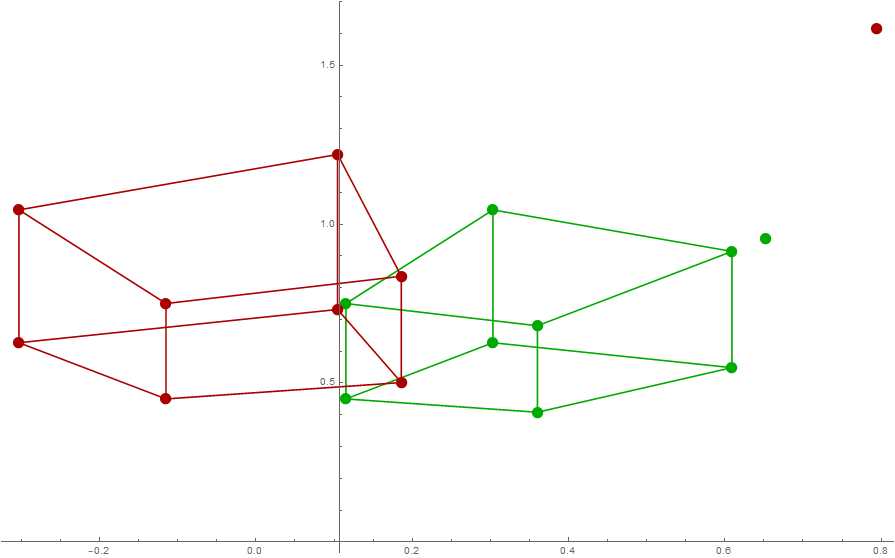
\includegraphics[width=.8\linewidth]{images/Rectification_one_same_Solutions.png}
	\caption[virtuelle Aufnahme eines Quaders für die Rektifizierung]{Aufnahmen zweier Kameras mit den selben Auflösungen, Kamera eins(Grün) und Kamera(rot) zwei gelten jeweils \ensuremath{\zeta =1}}
	\label{fig:RectOriginal} 
\end{figure}
\pagebreak

%\begin{minipage}{\linewidth}
%	\centering
%	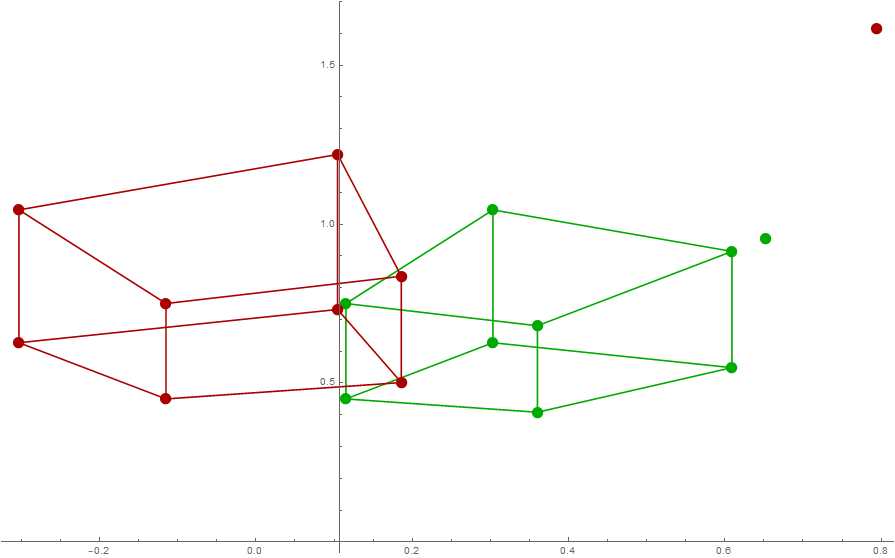
\includegraphics[width=.8\linewidth]{images/Rectification_one_same_Solutions.png}
%	\captionof{figure}{Aufnahmen zweier Kameras mit den selben Auflösungen, Kamera eins(Grün) und Kamera(rot) zwei gelten jeweils \ensuremath{\zeta =1}}
%	\label{fig:RectOriginal} 
%\end{minipage}\\ 

\begin{figure}[!htb]
	\centering
	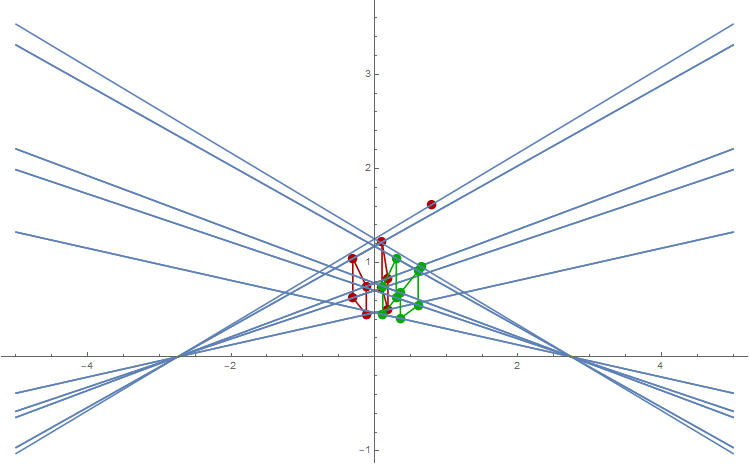
\includegraphics[width=.8\linewidth]{images/Rectification_two_same_Solutions.png}
	\caption[Epipolarlinien und Epipole vor der Rektifizierung]{Epipole für Kamera eins und Kamera zwei vor der Rektifizierung } 
	\label{fig:RectOriginalELines}
\end{figure}


%\begin{minipage}{\linewidth}
%	\centering
%	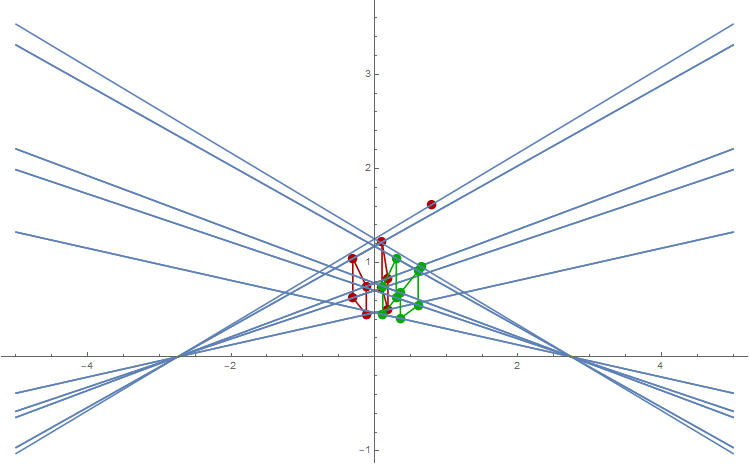
\includegraphics[width=.8\linewidth]{images/Rectification_two_same_Solutions.png}
%	\captionof{figure}{Epipole für Kamera eins und Kamera zwei vor der Rektifizierung } 
%	\label{fig:RectOriginalELines}
%\end{minipage}\\


Nach Transformieren der Abbildungspunkte mit den Matrizen $H_p$ und $H_p'$ wurden die Epipole ins unendliche Transformiert. Die Epipolarlinien verlaufen jetzt parallel zueinander, jedoch noch nicht zwingend parallel zur horizontalen Achse. In den Abbildung en \ref{fig:RectSameHp1} und \ref{fig:RectSameHp2} ist das Ergebnis der mit $H_p$ und $H_p'$ transformierten Bildpunkte zu sehen.

%Werden nun die Matritzen $H_p$ und $H_p'$ auf die jeweiligen Punkte der Bilder, $p_i$ für Bild eins und $p_j$ für Bild zwei, angewandt, so kann man eine erste Veränderung beobachten. Abbildung 4.9 zeigt beide Quader aus Abbildung 4.7 nachdem die jeweiligen Bildpunkte mit den projektiven Matrizen multipliziert wurden. Der Epipol in Bild eins bleibt natürlich wie zuvor im unendlichen, jedoch kann man erkennen, dass der rote Quader aus Bild zwei sich verändert hat. Sein Epipol wurde ins Unendliche transformiert und parallele Linien sind nun auch auf dem Bild parallel. Das die Epipolarlinien bereits horizontal parallel zur x-Achse verlaufen ist Zufall und ist nach der Anwendung der projektiven Matrizen auch noch nicht verlangt. Das Anpassen der Epipolarlinien, dazu gehört sie zunächst von beiden Bilder aus parallel zur x-Achse verlaufen zu lassen und dann noch sie so zueinander anzupassen, dass sie zu Scanlinien über beide Bilder verlaufen, verlgeiche Abbildung 4.12, folgt im nächsten Schritt. \\


%\begin{minipage}{\linewidth}
%	\centering
%	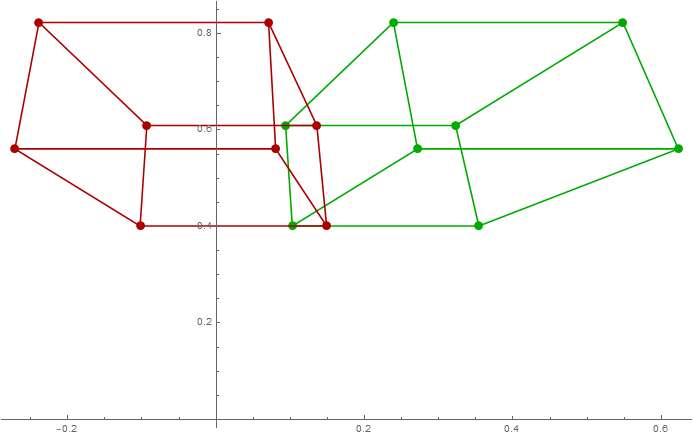
\includegraphics[width=1.\linewidth]{images/Rectification_Hp_same_Solutions.png}
%	\captionof{figure}{Abbildung beider Bilder nach anwenden der Matrizen $H_p$ und $H_p'$. Die Epipole beider Bilder sind nun im unendlichen.} 
%	\label{fig:RectSameHp}
%\end{minipage}\\ \\

\begin{figure}[!htb]
	\minipage{0.48\textwidth}
	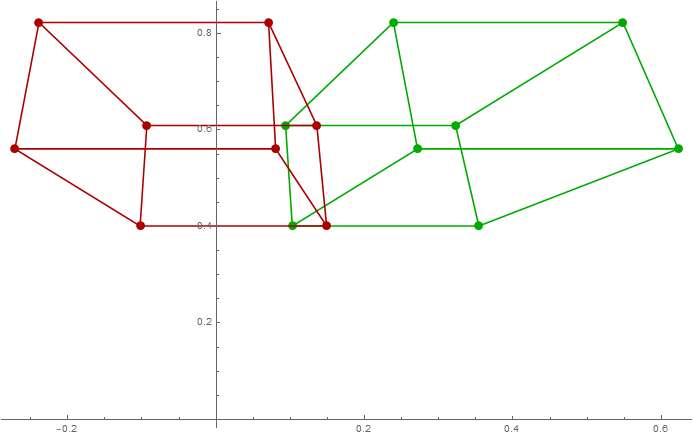
\includegraphics[width=\linewidth]{images/Rectification_Hp_same_Solutions.png}
	\caption[$H_p$ und $H_p'$ Transformation]{Abbildungen der Quader nach der Tranfromation mit $H_p$ und $H_p'$}
	\label{fig:RectSameHp1}
	\endminipage\hfill
	\minipage{0.48\textwidth}
	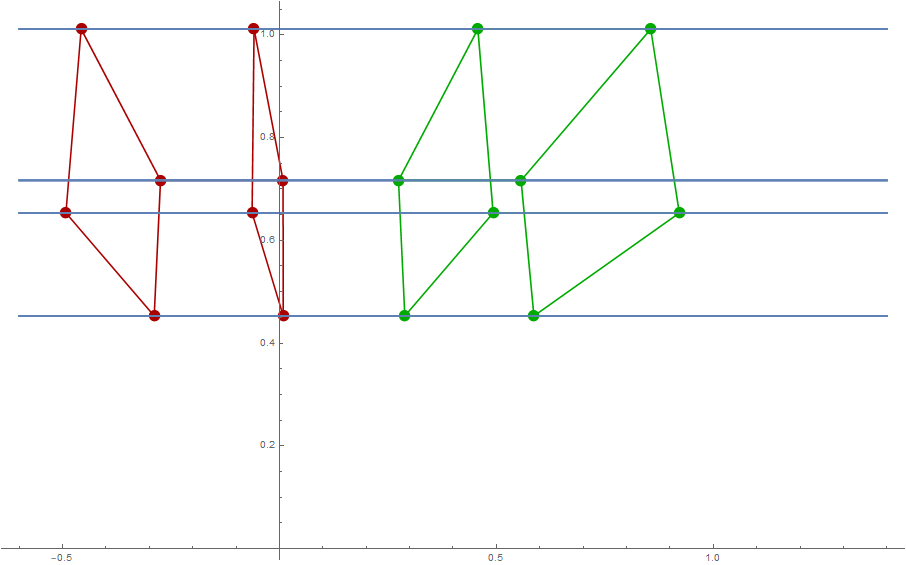
\includegraphics[width=\linewidth]{images/Rectification_Hp_same_Solutions_Lines.png}
	\caption[$H_p$ und $H_p'$ Transformation mit Epipolarlinien]{Abbildungen der Quader nach der Tranfromation mit $H_p$ und $H_p'$ mit eingezeichneten Epipolarlinien}
	\label{fig:RectSameHp2}
	\endminipage\hfill
	%\caption{Rekonstruierte Szene, wenn $K'$ mit einem Verhältnis von $[5:2]$ skaliert wurde}
	%\label{fig:RecT52}
\end{figure}

\subsection{Ähnlichkeitstransformation}



Die Epipole der jeweiligen Bilder befinden sich nach der projektiven Transformation im unendlichen. Die daraus resultierenden Epipolarlinien sind, wie in Abbildung \ref{fig:RectSameHp} zu sehen, parallel zueinander angeordnet. Im Folgenden sollen die Epipole rotiert werden, so dass sie ihre Richtungen $i = \begin{bmatrix}1&0&0\end{bmatrix}$ betragen. Die Epiplolarlinien würden dann parallel zur horizontalen Achse verlaufen\cite{ZZ}. $H_r$ und $H_r'$, welche aus der Zerlegung von $H_a$ und $H_a'$ resultieren, sollen die Rotation ausführen. Für $H_r$ und $H_r'$ gelten wie aus Gleichung \ref{eq:DefHr} bekannt folgende Gleichungen.

% dass die Richtung der Epipolarlinien $i = \begin{bmatrix}1&0&0\end{bmatrix}$ beträgt und sie parallel zu den horizontalen Achse verlaufen. 


%Nachdem die Epipole ins Unendliche verschoben wurden, müssen diese nun so rotiert und verschoben werden, dass die Epipolarlinien als Richtung $i = \begin{bmatrix}1&0&0\end{bmatrix}$ haben und die Epipolarlinien beider Bilder zu einheitlichen Scanlinien werden. Für die Ähnlichkeitstransformation wird davon ausgegangen, dass $w$ und $w'$ bereits bekannt sind.$H_r$ und $H_r'$ wurden bereits aus der Zerlegung von $H_a$ und $H_a'$ gewonnen. 

\begin{gather}
	H_r = 
	\begin{bmatrix}
		v_b-v_cw_b&	v_a-v_cw_a&0\\
		v_a-v_cw_a&v_b-v_cw_b&v_c\\
		0&0&1
	\end{bmatrix}\\
	H_r' = 
	\begin{bmatrix}
		v_b'-v_c'w_b'&	v_a'-v_c'w_a'&0\\
		v_a'-v_c'w_a'&v_b'-v_c'w_b'&v_c'\\
		0&0&1
	\end{bmatrix}
\end{gather}

$w$ und $w'$ sind bereits bekannt, Mit Hilfe von $F$, können $v_a$ und $v_b$ ersetzt werden. Zur Erinnerung eine Vorraussetzung für den hier aufgezeigten Rektifizierungsansatz ist, dass sowohl die Bildpunkte als auch die Fundamentalmatrix bekannt sein müssen. Die Fundamentalmatrix welche aus den rektifizierten Punkten entsteht hätte dann die Form 


\begin{gather}
	F = H'^T[i]_\times H\\
	F=
		\begin{bmatrix}
	u_a'&v_a'&w_a'\\
	u_b'&v_b'&w_b'\\
	u_c'&v_c'&1
	\end{bmatrix}
	\begin{bmatrix}
	0&0&0\\
	0&0&-1\\
	0&1&0
	\end{bmatrix} 
	\begin{bmatrix}
	u_a&u_b&u_c\\
	v_a&v_b&v_c\\
	w_a&w_b&1
	\end{bmatrix}\\
		F=
	\begin{bmatrix}
	v_aw_a' - v_a'w_a&v_bw_a' - v_a'w_b&v_cw_a' - v_a'\\
	v_aw_b' - v_b'w_a&v_bw_b' - v_b'w_b&v_cw_b' - v_b'\\
	v_a - v_c'w_a&v_b - v_c'w_b&v_c-v_c'
	\end{bmatrix}\\
\end{gather}

Da bisher nur $w$ und $w'$ bekannt sind und die Einträge der Fundamentalmatrix $F$ aus den nicht-rektifizierten Punkten, werden die Einträge so umgestellt. Für $v_a, v_b$ und $v_c$ werden jeweils die Einträge der letzten Zeile umgeformt. Für $v_a', v_b'$ und $v_c'$ dient die letzte Spalte von $F$.
%Dazu kann die letzte Zeile von F nach $v_a, v_b$ und $v_c$ aufgelöst werden. Für $v_a', v_b'$ und $v_c'$ wird die letzte Spalte von F verwendet. So können folgende Gleichungen für $v_a, v_a',v_b, v_b', v_c$ und $v_c'$ gewonnen werden. 


\begin{gather}
	v_a = F_{31}+v_c'w_a\label{eq:va}\\
	v_b = F_{32}+v_c'w_b\\
	v_c = F_{33}+v_c'\\
	v_a' = v_cw_a'-F_{13}\\
	v_b' = v_cw_b'-F_{23}\\
	v_c' = v_c -F_{33}\label{eq:F33}
\end{gather}

$F_{31},\, F_{32}, F_{33} ,F_{13}$ und  $F_{23}$ stehen für die Einträge der Matrix $F$, welche aus den nicht-rektifizierten Punkten bestimmt wurde. \\


Werden die Gleichungen \ref{eq:va} bis \ref{eq:F33} in $H_r$ und $H_r'$ eingesetzt, so ergeben sich für $H_r$ und $H_r'$ 

%Eingesetzt in die jeweiligen Matrizen $H_r$ und $H_r'$, entstehen die folgenden Matrizen in Gleichungen 4.114 und 4.115, welche nur noch die unbekannte $v_c'$ beinhalten. Die gemeinsame Variable $v_c'$ zeigt die geometrische Verbindung beider Bilder in ihrer Verschiebung entlang ihrer v-Richtung. Es wird also ein Offset von $F_33$ benötigt, um die Epipolarlinien horizontal zu Scanlinien auszurichten. \textcolor{red}{Den Wert für $v_c$ wird so ermittelt, dass das Minimum einer v-Koordinaten eines Pixel als minimum den Wert null besitzt }

\begin{gather}
	H_r = \begin{bmatrix}
		F_{32}-w_bF_{33}&w_aF_{33}-F_{31}&0\\
		F_{31}-w_aF_{33}&F_{32}-w_bF_{33}&F_{33}+v_c'\\
		0&0&1
	\end{bmatrix}\\
	H_r'=
	\begin{bmatrix}
		w_b'F_{33}-F_{23}&F_{13}-w_a'F_{33}&0\\
		w_a'F_{33}-F_{13}&w_b'F_{33}-F_{23}&v_c'\\
		0&0&1
	\end{bmatrix}
\end{gather}\\


Die gemeinsame unbekannte Variable $v_c'$ beschreibt die geometrische Verbindung beider Bilder in ihrer Verschiebung entlang ihrer vertikalen Richtung\cite{ZZ}. $F_33$ ist somit der horizontale Versatz, welcher benötigt wird, um die horizontalen Epipolarlinien beider Bilder zueinander auszurichten, so dass die gewünschten Scanlinien über beide Bilder entstehen. $v'$ wird dabei so gewählt, dass die kleinste Koordinate der rektifizierten Bilder in vertikaler Achsenrichtung gleich null ist.\cite{ZZ}.\\


%
% Es wird also ein Offset von $F_33$ benötigt, um die Epipolarlinien horizontal zu Scanlinien auszurichten. \textcolor{red}{Den Wert für $v_c$ wird so ermittelt, dass das Minimum einer v-Koordinaten eines Pixel als minimum den Wert null besitzt }

Die Abbilder des Quader sehen nach der Transformation mit $H_rH_p$ und $H_r'H_p'$ aus wie in den Abbildungen \ref{fig:RectSameHrHp1} und \ref{fig:RectSameHrHp2} dargestellt. Sollten die Epipolarlinien noch nicht parallel zur horizontalen Achse gewesen sein, so sind sie es nach der Transformation mit $H_p$ und $H_p'$. Des Weiteren wurden beide Bilder durch $v_c'$ so verschoben, dass der in vertikaler Richtung kleinste Punkt bei auf der Horizontalen Achse liegt. 
%Das Ergebnis der Bildpunkte $p_i$ und $p_j$ multipliziert mit den Matrizen $H_rH_p$ und $H_r'H_p'$ mit ist in Abbildung 4.10 zu sehen. Als letztes folgt noch die Scherungstransformation $H_s$ und $H_s'$ für die horizontale Entzerrung beider Bilder.\\ 

%\begin{minipage}{\linewidth}
%	\centering
%	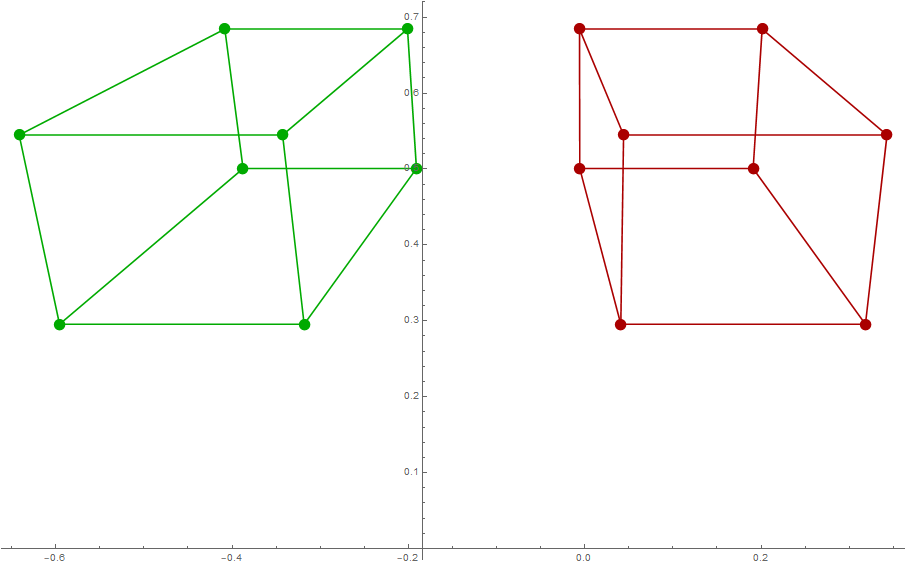
\includegraphics[width=1.\linewidth]{images/Rectification_HrHp_same_Solutions.png}
%	\captionof{figure}{Abbildung beider Bilder nach anwenden der Matrizen $H_r \cdot H_p$ und $H_r' \cdot H_p'$. Die Epipolarlinien sind nun horizontal zueinander ausgerichtet} 
%	\label{fig:RectSameHrHp}
%\end{minipage}\\ \\

\begin{figure}[!htb]
	\minipage{0.48\textwidth}
	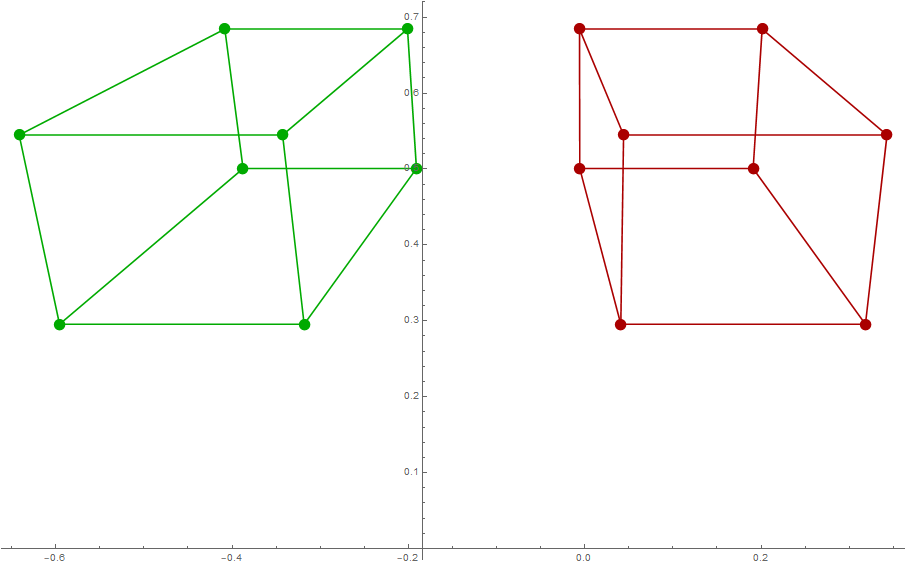
\includegraphics[width=\linewidth]{images/Rectification_HrHp_same_Solutions.png}
	\caption[$H_rH_p$ und $H_r'H_p'$ Transformation]{Abbildungen der Quader nach der Tranfromation mit $H_rH_p$ und $H_r'H_p'$}
	\label{fig:RectSameHrHp1}
	\endminipage\hfill
	\minipage{0.48\textwidth}
	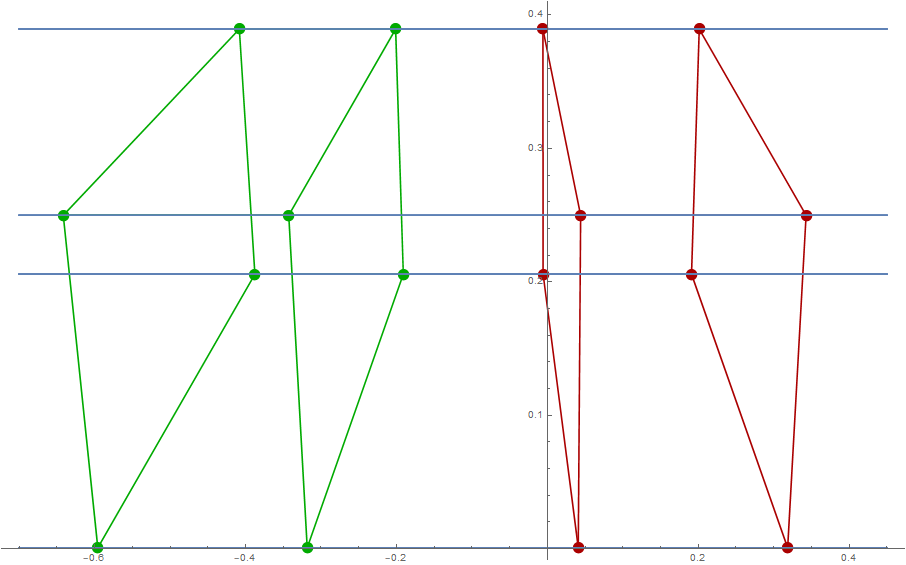
\includegraphics[width=\linewidth]{images/Rectification_HrHp_same_Solutions_Lines.png}
	\caption[$H_rH_p$ und $H_r'H_p'$ Transformation mit Epipolarlinien]{Abbildungen der Quader nach der Tranfromation mit $H_rH_p$ und $H_r'H_p'$ mit eingezeichneten Epipolarlinien}
	\label{fig:RectSameHrHp2}
	\endminipage\hfill
	%\caption{Rekonstruierte Szene, wenn $K'$ mit einem Verhältnis von $[5:2]$ skaliert wurde}
	%\label{fig:RecT52}
\end{figure}


\subsection{Scherungstransformation}

Im letzten Schritt soll die durch die Transformation mit $H_p$ und $H_p'$ entstandene horizontale Verzerrung in beiden Bilder reduziert werden. Aus diesem Grund werden die Scherungsmatrizen $H_s$ und $H_s'$, aus der Zerlegung der affinen Matrix $H_a$ und $H_a'$ benötigt. Die Einträge der ersten zeile in $H_s$ und $H_s'$ haben nur noch Auswirkungen auf die horizontalen Koordinaten der Bildpunkte.

%Die letzte Transformation, welche an den Bilder durchgeführt werden soll, ist die sogenannten Scherungstransformation. Sie soll vor allem dazu dienen, die horizontale Verzerrung der Bilder, zueinander nochmal weiter zu minimieren. Die Matrizen $H_s$ und $H'_r$ wirken sich hauptsächlich auf die $u$ und $u'$ Komponenten aus. 

\begin{gather}
	H_s =\begin{bmatrix}
		u_a&u_b&0\\
		0&1&0\\
		0&0&1
	\end{bmatrix}\\
	H'_s =\begin{bmatrix}
		u'_a&u'_b&0\\
		0&1&0\\
		0&0&1
	\end{bmatrix}
\end{gather}

Um die richtigen Werte für $a, a', b$ und $b'$ zu bekommen, werden zunächst Punkte an den jeweiligen gegenüberliegenden Kanten der Bilder definiert. Da die Bilder des Quaders nicht aus tausenden von Pixeln bestehen, wie ein reales Bild, sondern nur über dessen Eckpunkte bestimmt ist, wird eine Bildbreite $w$ und $w'$ und eine Bildhöhe $h$ und $h'$ definiert. \\

Da es nicht möglich ist die horizontale Verzerrung gänzlich zu reduzieren, wird stattdessen versucht die Orthogonalität und das Seitenverhältnis der Verbindungslinien $\overline{bd}$ und $\overline{ca}$ wieder herzustellen. In Abbildung \ref{fig:PreserveAspectRatio} ist das Ziel nochmal grafisch dargestellt.\\

Für den nächsten Schritt werden im synthetischen Beispiel für die Abbildungen des Quaders jeweils Bildweite $w$ und Bildhöhe $h$ definiert. Da zunächst von gleichen Kameraauflösungen ausgegangen wird, sind die Bildbreiten und Höhen beider Kameras gleich. Danach werden die vier Mittelpunkte $a,b,c$ und $d$ der Bildkanten definiert mit $a = [\frac{w-1}{2} \; 0 \; 1]^T, b = [w-1 \; \frac{h-1}{2}\; 1]^T, c = [\frac{w-1}{2} \; h-1 \; 1]^T, d = [0 \; \frac{h-1}{2} \; 1]^T$.



\begin{figure}[!htb]
	\centering
	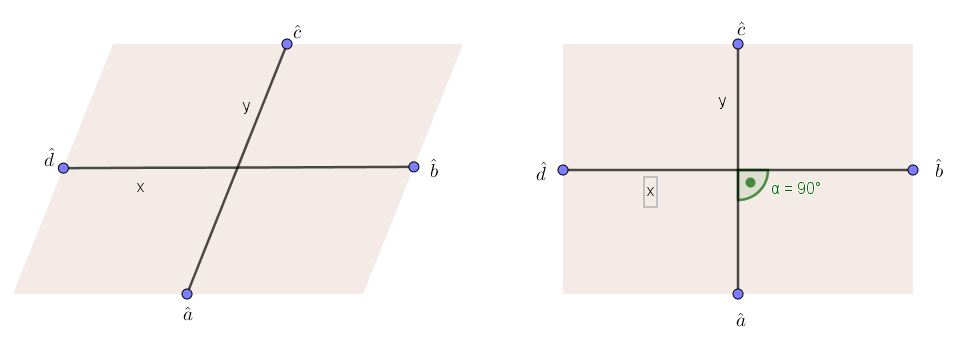
\includegraphics[width=.8\linewidth]{images/Scherungstransformation.png}
	\caption[Wiederherstellung der Orthogonalität]{Die Verbindungslinien  $\overline{bd}$ und $\overline{ca}$ sollen so ausgerichtet werden, dass sie orthogonal zueinander stehen.} 
	\label{fig:PreserveAspectRatio}
\end{figure}

Die Punkte $a,b,c,d$ und auch $a',b',c',d'$ sind die Mittelpunkte der noch nicht rektifizierten Bildkanten. Diese werden mit den Transformationsmatrizen $H_sH_rH_p$ und $H_s'H_r'H_p'$ verrechnet, um so die Position der Kantenmitten nach der Rektiizierung zu erhalten.

%geben die Bildbreiten der noch unberührten Bilder an. Nach der Rektifizierung sind die Bilder so verzerrt, dass die Kanten mitten sich meistens nicht mehr direkt gegenüber von einander befinden. Die Punkte $a,b,c,d$ und $a',b',c',d'$ werden mit den Matrizen $H_p, H'_p, H_r$ und $H'_r$ verrechnet, so dass man die genaue neue Position der Kanten Mitten nach der Rektifizierung hat. 

\begin{gather*}
	\hat{a} = H_r\cdot H_p \cdot a\\
	\hat{b} = H_r\cdot H_p \cdot b\\
	\hat{c} = H_r\cdot H_p \cdot c\\
	\hat{d} = H_r\cdot H_p \cdot d\\
	\hat{a'} = H'_r\cdot H'_p \cdot a'\\
	\hat{b'} = H'_r\cdot H'_p \cdot b'\\
	\hat{c'} = H'_r\cdot H'_p \cdot c'\\
	\hat{d'} = H'_r\cdot H'_p \cdot d'\\
\end{gather*}

%Um aus $\hat{a},\hat{b},\hat{c},\hat{d}$ und auch $\hat{a}',\hat{b}',\hat{c}',\hat{d}'$ wieder Punkte der affinen Ebene zu machen werden sie jeweils durch ihre dritte Komponenten geteilt, so das $\hat{a}_w,\hat{b}_w,\hat{c}_w,\hat{d}_w$ und $\hat{a}'_w,\hat{b}'_w,\hat{c}'_w,\hat{d}'_w$ jeweils den Wert eins besitzen. 

Danach können die Vektoren $\vec{x}$ und $\vec{y}$ aus den Differenzen der sich ursprünglich gegenüberliegenden Punkte gebildet werden.

\begin{gather}
	x = \hat{b}-\hat{d}\\
	y = \hat{c}-\hat{a}\\
	x' = \hat{b}'-\hat{d}'\\
	y' = \hat{c}'-\hat{a}'
\end{gather}

$x$ und $y$ sind Vektoren der euklidischen Bildebene\cite{ZZ}. Das heißt, sie sind genau dann orthogonal zueinander wenn gilt:

\begin{gather}
	(H_sx)^T(H_sy)= 0 \label{eq:OrthoHs}\\
	(H'_sx')^T(H'_sy')= 0 \label{eq:OrthoHs2}
\end{gather}

Für die Erhaltung der Seitenverhältnisse gilt dann:

\begin{gather}
	\frac{(H_sx)^T(H_sx)}{(H_sy)^T(H_sy)} = \frac{w^2}{h^2} \label{eq:SeitenverhaeltnisHs}\\
	\frac{(H'_sx')^T(H'_sx')}{(H'_sy')^T(H'_sy')} = \frac{w'^2}{h'^2}\label{eq:SeitenverhaeltnisHs2}	
\end{gather}

Anhand der in den Gleichungen \ref{eq:OrthoHs}, \ref{eq:OrthoHs2}, \ref{eq:SeitenverhaeltnisHs} und \ref{eq:SeitenverhaeltnisHs2} können die folgenden Gleichungen für die Matirixeinträge für $H_s$ und $H_s'$ aufgestellt werden\cite{ZZ,ACM}.


\begin{gather}
u_a = \frac{h^2x_v^2+w^2+y_v^2}{hw(x_vy_u-x_uy_v)}\\
u_b = \frac{h^2x_ux_v+w^2y_uy_v}{hw(x_uy_v-x_vy_u)}
\end{gather}

%Für $u_a, u'_a, u_b$ und $u'_b$ jeweils Gleichungen auf Basis der jeweiligen Bild Höhen und Breiten $w,w',h,h'$ und $x,x',y$ und $y'$ und unter Einhaltung der Aussagen der Gleichungen 5.118 bis 5.121, aufgestellt werden\cite{ZZ,ACM}. 

Die selben Gleichungen werden auch für $u'_a$ und $u'_b$ aufgestellt. Das Ergebnis der gesammten Transformation $H$ mit $H_sH_rH_p$ und $H'$ mit $H_s'H_r'H_p'$ ist in den Abbildungen \ref{fig:RectSameHsHrHp1} und \ref{fig:RectSameHsHrHp2} zu sehen.\\

%Das Ergebnis der Scherungstransformation ist in Abbildung 5.17 dargestellt. \textcolor{red}{ Wie zu sehen ist, ist die Minimierung noch nicht zu hindert prozent perfekt, hierfür müsste man noch ein paar mehr Interationsschritte bei finden von $z$ einfügen.}(ICH WEIß GANZ EHRLICH NICHT WORAN ES LIEGT...)


%\begin{minipage}{\linewidth}
%	\centering
%	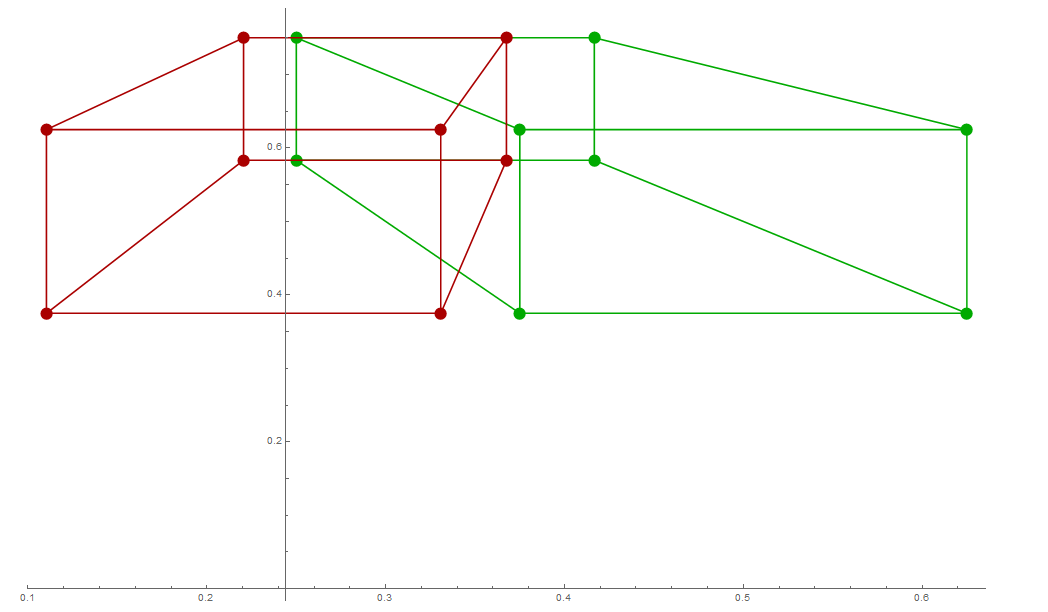
\includegraphics[width=1.\linewidth]{images/Rectification_HsHrHp_same_Solutions.png}
%	\captionof{figure}{Abbildung beider Bilder nach anwenden der Matrizen $H_s \cdot H_r \cdot H_p$ und $H_s' \cdot H_r' \cdot H_p'$. Die horizontale Verzerrung wurde reduziert.} 
%\end{minipage}\\ \\
%
%\begin{minipage}{\linewidth}
%	\centering
%	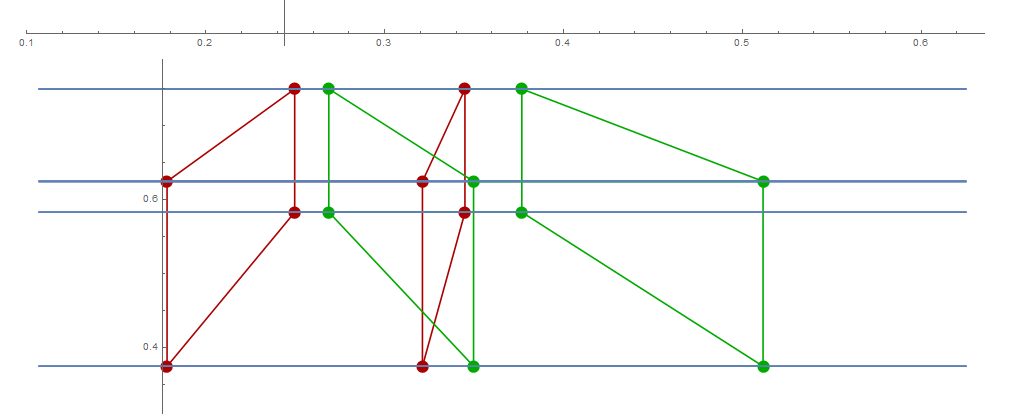
\includegraphics[width=1.\linewidth]{images/Rectification_four_same_Solutions.png}
%	\captionof{figure}{In dieser Abbildung wurden die Epipolarlinien noch in den Grafikplot mit eingebaut} 
%\end{minipage}\\ \\


\begin{figure}[!htb]
	\minipage{0.48\textwidth}
	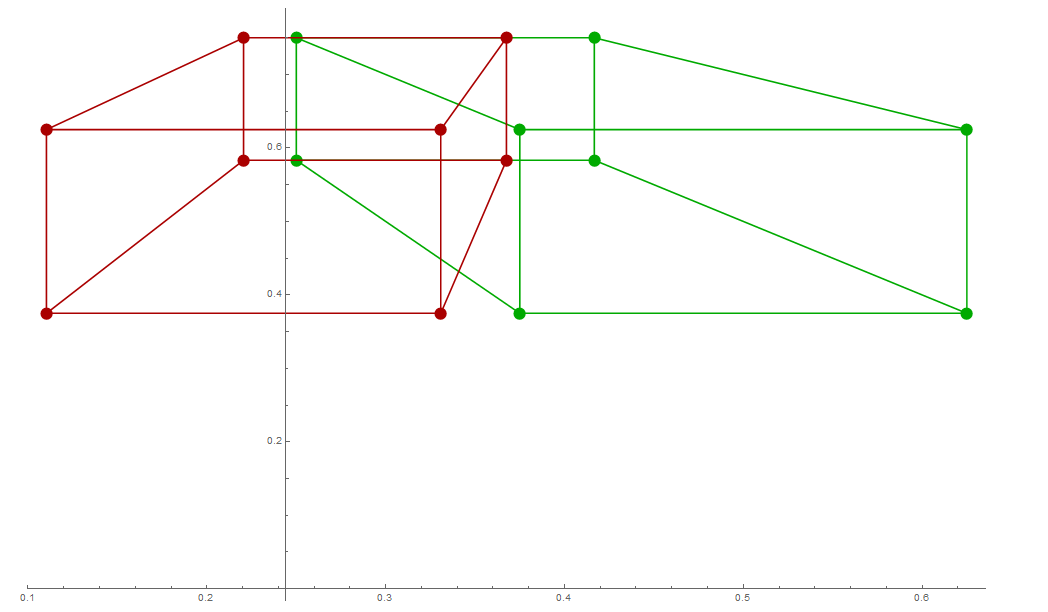
\includegraphics[width=\linewidth]{images/Rectification_HsHrHp_same_Solutions.png}
	\caption[$H_sH_rH_p$ und $H_s'H_r'H_p'$ Transformation]{Abbildungen der Quader nach der Tranfromation mit $H_sH_rH_p$ und $H_s'H_r'H_p'$}
	\label{fig:RectSameHsHrHp1}
	\endminipage\hfill
	\minipage{0.48\textwidth}
	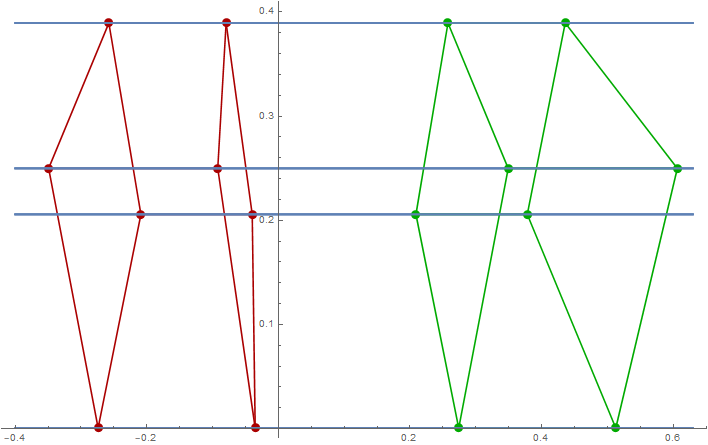
\includegraphics[width=\linewidth]{images/Rectification_HsHrHp_same_Solutions_Lines.png}
	\caption[$H_sH_rH_p$ und $H_s'H_r'H_p'$ Transformation mit Epipolarlinien]{Abbildungen der Quader nach der Tranfromation mit $H_sH_rH_p$ und $H_s'H_r'H_p'$ mit eingezeichneten Epipolarlinien}
	\label{fig:RectSameHsHrHp2}
	\endminipage\hfill
	%\caption{Rekonstruierte Szene, wenn $K'$ mit einem Verhältnis von $[5:2]$ skaliert wurde}
	%\label{fig:RecT52}
\end{figure}

\section{Rektifizierung mit unterschiedlichen Kamerauflösungen}


Im Folgenden wird der entstandenen Rektifizierungsalgorithmus auf Bilder unterschiedlicher Auflösung angewandt. Im ersten Beispiel wird für $C$ die Auflösung $\zeta_x = \zeta_y =1$ gewählt. Die Kameramatrix $K$ lautet wie folgt


\begin{gather}
	K = 
	\begin{bmatrix}
	1&0&0\\
	0&1&0\\
	0&0&1
	\end{bmatrix}
\end{gather}

Für $C'$ wird eine kleinere Auflösung mit $\zeta'_x = \zeta'_y = 0.5$ definiert. Die Kameramatrix $K'$ lautet somit

\begin{gather}
	\begin{bmatrix}
	0.5&0&0\\
	0&0.5&0\\
	0&0&1
	\end{bmatrix}
\end{gather} 


Die entstehenden Bilder des Quaders sind in Abbildung \ref{fig:AbbRecDifRes} zu sehen. Da $K'$ nur eine halb so große Auflösung wie $K$ besitzt, ist das resultierende Bild des roten Quaders auch nur halb so groß. Der grüne Quader zeigt das entstehende Bild von $C'$.
\pagebreak

\begin{figure}[!htb]
	\centering
	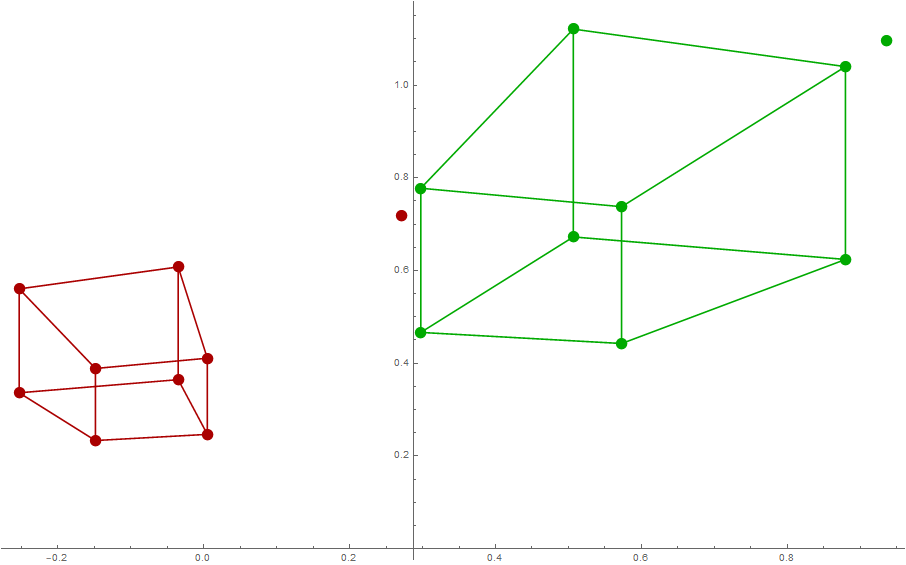
\includegraphics[width=1.\linewidth]{images/Rectification_one_different_Solutions.png}
	\caption[virtuelle Aufnahme mit unterschiedlichen Auflösung für die Rektifizierung]{Aufnahmen zweier Kameras mit unterschiedlichen Auflösungen.Für Kamera eins(Grün) gilt \ensuremath{\zeta_x = \zeta_y = 1}  und für Kamera zwei(rot) gilt \ensuremath{\zeta'_x = \zeta'_y= 2}.} 
	\label{fig:AbbRecDifRes}
\end{figure}


%\begin{minipage}{\linewidth}
%	\centering
%	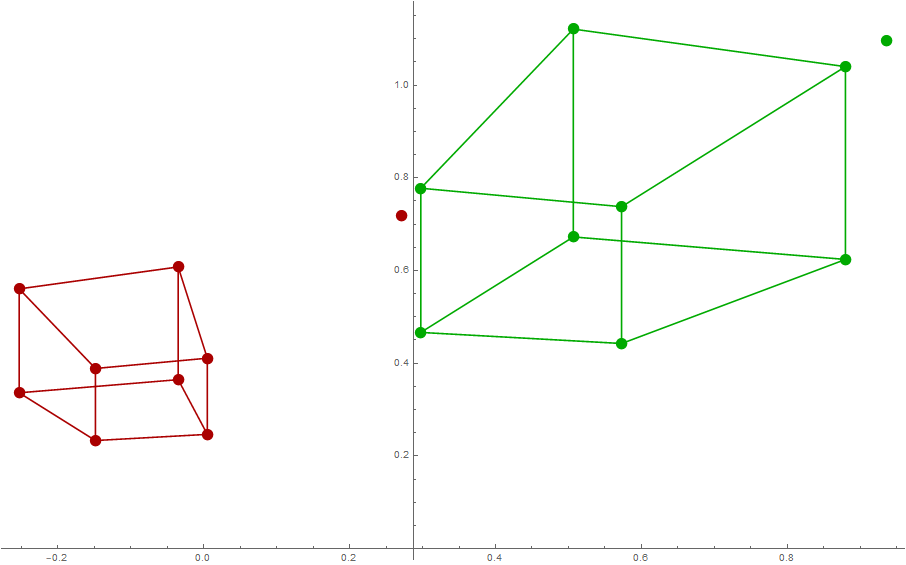
\includegraphics[width=1.\linewidth]{images/Rectification_one_different_Solutions.png}
%	\captionof{figure}{Aufnahmen zweier Kameras mit unterschiedlichen Auflösungen.Für Kamera eins(Grün) gilt \ensuremath{\zeta_x = \zeta_y = 1}  und für Kamera zwei(rot) gilt \ensuremath{\zeta'_x = \zeta'_y= 2}.} 
%	\label{fig:AbbRecDifRes}
%\end{minipage}\\ \\

Abbildung \ref{fig:AbbRecDifResHp} zeigt die projektive Transformation der beiden Bilder mit $H_p$ und $H_p'$. Die Epipolarlinien der beiden Bilder sind nach dieser Transformation jeweils parallel zueinander. In Abbildung \ref{fig:AbbRecDifResHrHp} ist das Resultat zu sehen wenn die Transformation $H_r$ und $H_r'$ dazukommen. Die Epipolarlinien sind jetzt parallel zur horizontalen Achse und die Epipolarlinien von Bild eins und Bild zwei sind so zueinander ausgerichtet, dass sie zu einheitlichen Linien über zwei Bilder werden. Der rote Quader, welches das Bild mit der niedrigeren Auflösung repräsentiert, ist nach dieser Transformation stark horizontaler und vertikaler Richtung vergrößert wird. 
%(Normalerweise in realbildern wird das bild bei unterschiedlicher Auflösung nicht verzerrt sondern nur "Vergrößert" oder zurecht "geschnitten". Dadruch dass beide Quader in einem Koordinatensystem verbaut wurden sieht das so aus)


\begin{figure}[!htb]
	\minipage{0.48\textwidth}
	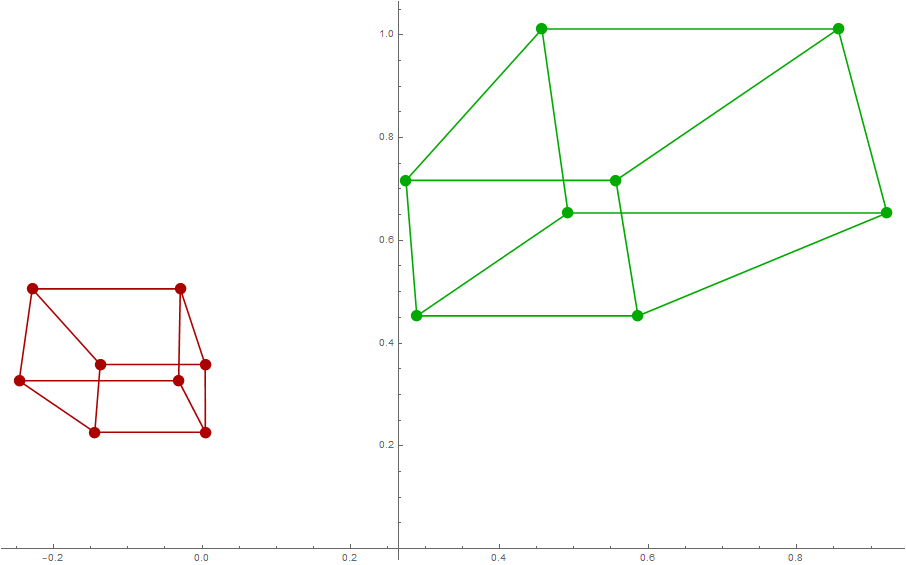
\includegraphics[width=\linewidth]{images/Rectification_Hp_different_Solutions.png}
	\caption[Transformation $H_p$ und $H_p'$ angewandt auf Bilder unterschiedlicher Auflösungen]{Transformation $H_p$ und $H_p'$ angewandt auf Bilder unterschiedlicher Auflösungen}
	\label{fig:AbbRecDifResHp}
	\endminipage\hfill
	\minipage{0.48\textwidth}
	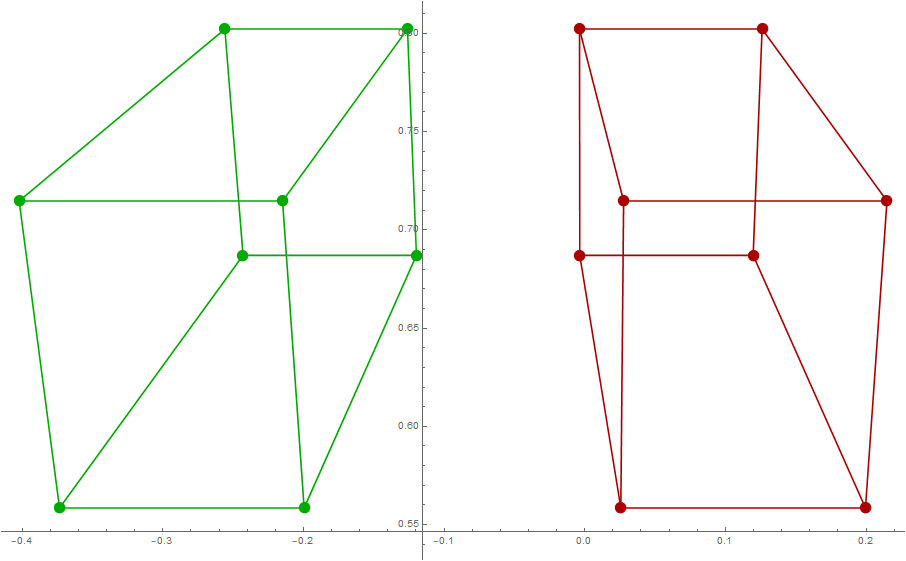
\includegraphics[width=\linewidth]{images/Rectification_HrHp_different_Solutions.png}
	\caption[Transformation $H_rH_p$ und $H_r'H_p'$ angewandt auf Bilder unterschiedlicher Auflösungen]{Transformation $H_rH_p$ und $H_r'H_p'$ angewandt auf Bilder unterschiedlicher Auflösungen}
	\label{fig:AbbRecDifResHrHp}
	\endminipage\hfill
	%\caption{Rekonstruierte Szene, wenn $K'$ mit einem Verhältnis von $[5:2]$ skaliert wurde}
	%\label{fig:RecT52}
\end{figure}

Die Abbildungen \ref{fig:AbbRecDifResHsHrHp} und \ref{fig:AbbRecDifResHsHrHpLines} zeigen die letzt Transformation mit $H_s$ und $H_s'$ einmal mit und einmal ohne Epipolarlinien. Die Bilder scheinen richtig rektifiziert geworden zu sein. Dieser Test wurde noch mit weiteren Vielfachen der Kameramatrix $K$ ausprbiert, immer mit dem selben Ergebnis wie in den Abbildungen \ref{fig:AbbRecDifResHsHrHp} und \ref{fig:AbbRecDifResHsHrHpLines} zu sehen. Somit ist es wohl prinzipiell möglich aus den Rektifizeriten Bilder eine Tiefenkarte zu erstellen und somit die 3D-Szene zu rekonstruieren.\\


\begin{figure}[!htb]
	\minipage{0.48\textwidth}
	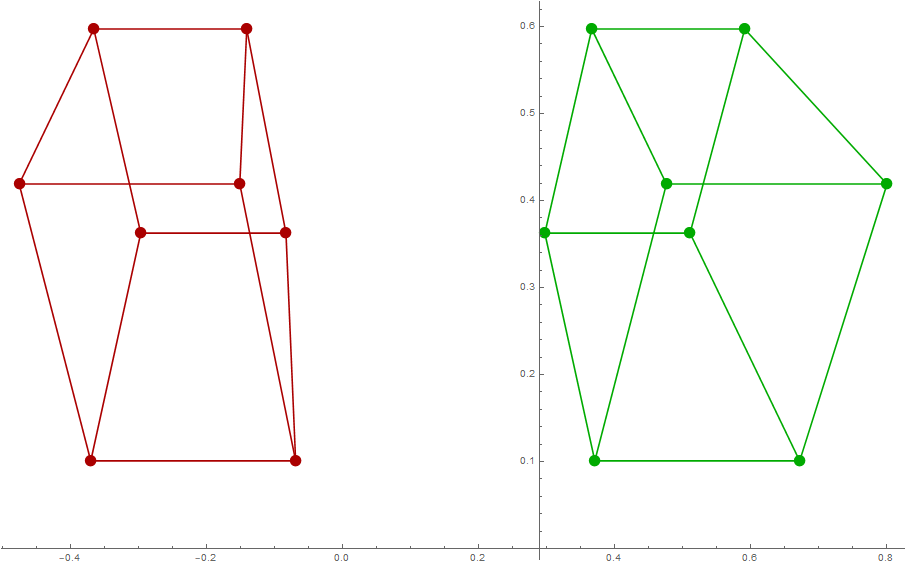
\includegraphics[width=\linewidth]{images/Rectification_HsHrHp_different_Solutions.png}
	\caption[Transformation $H_sH_rH_p$ und $H_s'H_r'H_p'$ bei unterschiedlicher Auflösungen]{Transformation $H_sH_rH_p$ und $H_s'H_r'H_p'$ angewandt auf Bilder unterschiedlicher Auflösungen}
	\label{fig:AbbRecDifResHsHrHp}
	\endminipage\hfill
	\minipage{0.48\textwidth}		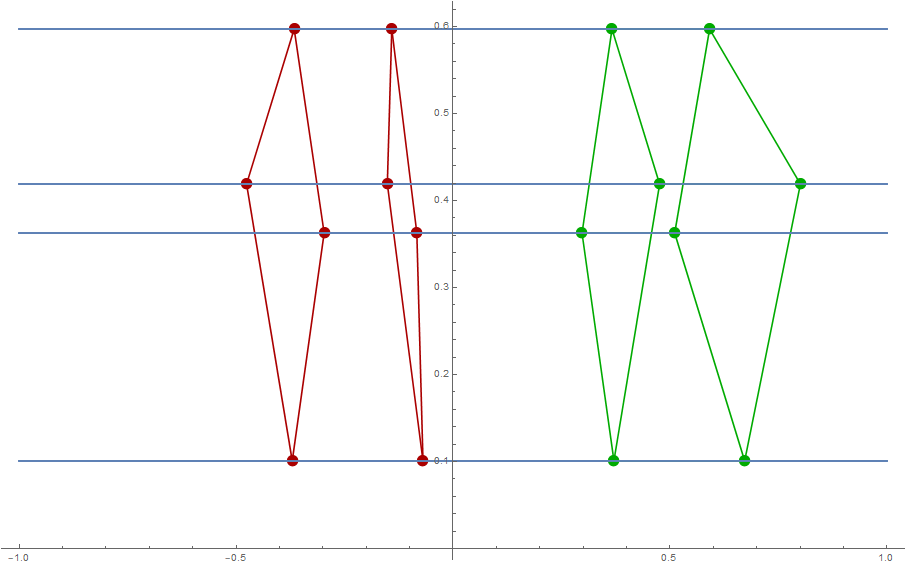
\includegraphics[width=\linewidth]{images/Rectification_four_different_Solutions.png}
	\caption[Transformation $H_sH_rH_p$ und $H_s'H_r'H_p'$ mit Epipolarlinien]{[Transformation $H_sH_rH_p$ und $H_s'H_r'H_p'$ angewandt auf Bilder unterschiedlicher Auflösungen mit Epipolarlinien}
	\label{fig:AbbRecDifResHsHrHpLines}
	\endminipage\hfill
		%\caption{Rekonstruierte Szene, wenn $K'$ mit einem Verhältnis von $[5:2]$ skaliert wurde}
		%\label{fig:RecT52}
\end{figure}



Als nächstes wurden die Auflösung von $C'$ so verändert, dass $\zeta'_x \neq \zeta'_y$ gilt. Es werden $\zeta'_x = 2.3$  und $\zeta'_y = 3.2$ definiert. Somit folgt für $K'$ die folgende Matrix.

\begin{gather}
	K' = 
	\begin{bmatrix}
	2.3&0&0\\
	0&3.2&0\\
	0&0&1
	\end{bmatrix}
\end{gather}

Für $K$ von $C$ gilt weiterhin $\zeta_x = \zeta_y = 1$. Die Entstehenden Bilder sind in Abbildung \ref{fig:7.18} zu sehen. Die horizontale Kantenlänge roten Quaders ist im Verhältnis kürzer als ihre vertikale Kantenlänge. Wie in Abbildung \ref{fig:7.19} zu sehen ist, bleibt ungleiche Veränderte Seitenverhältnis des roten Quaders nach der Rektifizierung erhalten, weshalb der Rote Quader schmäler ist als der der grüne.


\begin{figure}[!htb]
	\minipage{0.48\textwidth}
	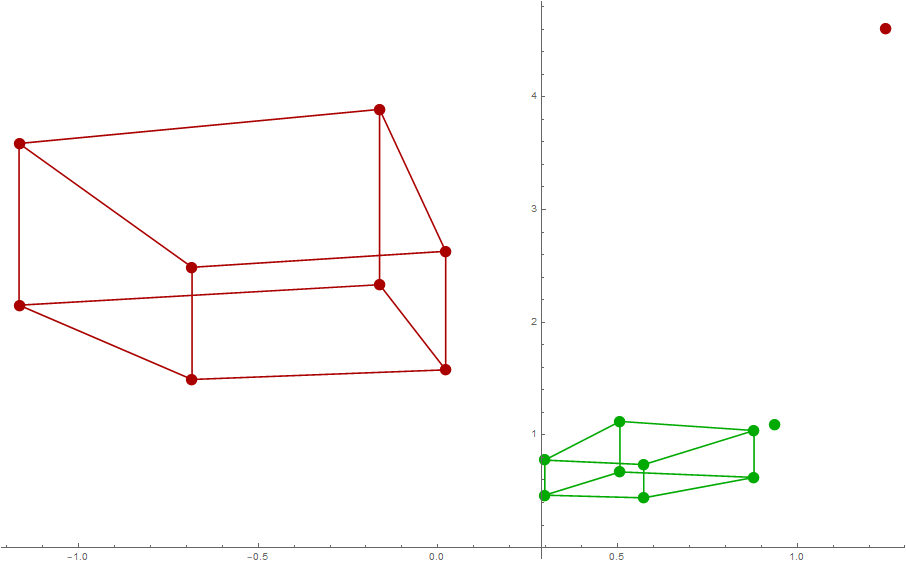
\includegraphics[width=\linewidth]{images/Rectification_Resolution_Abbild_verhaeltnisse.png}
	\caption[Rektifizierung mit $\zeta'_x = 2.3$ und $\zeta'_y = 3.2$]{Aufnahmen zweier Kameras mit unterschiedlichen Auflösungen.Für Kamera eins(grün) gilt \ensuremath{\zeta_x = \zeta_y = 1}  und für Kamera zwei(rot) gilt \ensuremath{\zeta'_x = 2.3} $\zeta'_y= 3.2$}
	\label{fig:7.18}
	\endminipage\hfill
	\minipage{0.48\textwidth}
	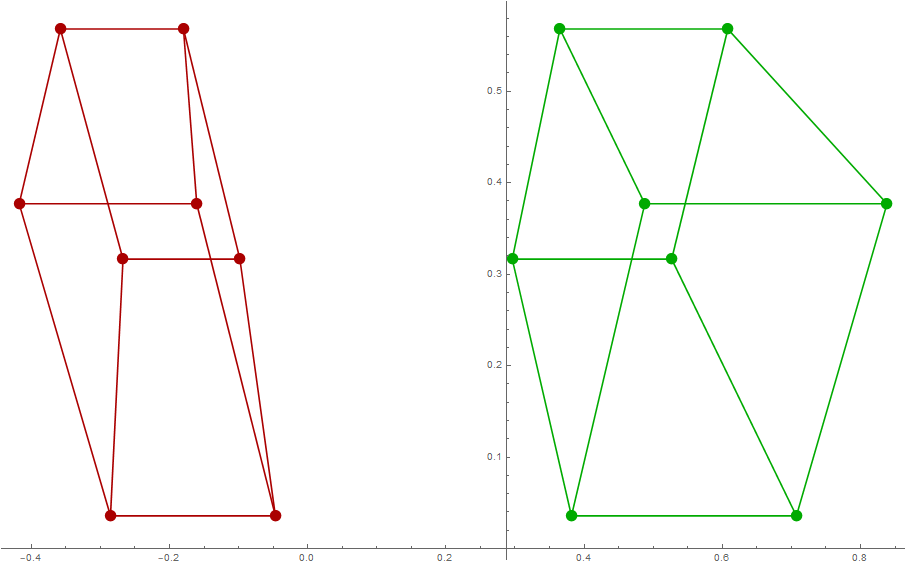
\includegraphics[width=\linewidth]{images/Rectification_Resolution_verhaeltnisse.png}
	\caption[Rektifizierung mit $\zeta'_x = 2.3$ und $\zeta'_y = 3.2$]{Nach der Rektifizierung stimmen die horizontalen Koordinaten nicht überein, es würde zu Fehlern in der Tiefenkarte und somit in der gesamten 3D-Rekonstruktion geben.}
	\label{fig:7.19}
	\endminipage\hfill
	%\caption{Rekonstruierte Szene, wenn $K'$ mit einem Verhältnis von $[5:2]$ skaliert wurde}
	%\label{fig:RecT52}
\end{figure}

Die Beispiele zeigen, dass es möglich ist Bilder unterschiedlicher Beispiele zu rektifizieren, jedoch müssen für die nachfolgende Erstellung der Tiefenmaps....(was wäre jetzt ein guter Abschluss??)
